
\chapter{Model cardiac cells at tissue and whole-heart level}
\label{chap:model-cardiac-cells}

The heart is composed of discrete cells in which each cell is an excitable
system. At the microscopic level, it's quite complicated that cardiac muscle is
a composite tissues with different cell types, mainly myocytes
(endocardium, M-cells (Masonic, Midmyocardial, Moe), epicardium) and
fibroblasts, supported by extracellular matrix (ECM) and permeated by fluids.
The detailed models of a single myocyte are still under actively development
(see Part.\ref{part:compartmental_model}, and Part.\ref{part:spatial_modeling}).
Compartmental models requires using ODE while temporo-spatial models require
solving PDEs which need significant computational powers.

In many ways, a model would help compliment the experimental and clinical
studies that seeks to elucidate the mechanism of arrhythmogenesis (the development of an
arrhythmia). A more realistic model combines the knowledge from physics,
mathematics, biomedical engineering, cardiology, and computer science. The
question we aims to answer is to study the factors contributing to {\it
conduction failure} or {\it rhythm instability}. This can be done at the tissue
or whole-heart level.


\section{Papers to read}

\citep{spach1995}


\section{Introduction}

On average a mature young (17-30 years) healthy human heart contains about 6.5
billion cells in the ventricles \citep{clayton2010}, based on the fact that
8.2billion myocyte nuclei was found \citep{olivetti1991}, and the assumption
that 25\% of cells have two nuclei and 75\% percent one nucleus
\citep{olivetti1996}.
Every year, about 52 milion ventricular myocyte nuclei was lost to ensure a
subsequently increase in ventricular myocyte volume of 110-120$\mu^3$ per year
\citep{olivetti1991} to preserve the thickness. As a matter of fact, most tissue
and whole-heart models use a very simple single-cardiac cell model, or even
ignore individual cells, but consider the heart as the structure of two
separated but continuous medium: intracellular spaces and extracellular space
like {\it bidomain} model approach; or only the intracellular space (like {\it
monodomain} model approach).


Research groups:
\begin{enumerate}
  \item IBM Watson: Cardioid Heart Modelling Project
  \url{http://researcher.watson.ibm.com/researcher/view_project.php?id=2992#Tissuelevel}
  \item Trayanova at JHU: 3D electromechanical model of ventricular contraction
  with anatomically accurate geometry derived from structural imaging data.
  \item CMISS (Univ.Auckland, NZ): \url{www.cmiss.org/openCMISS}
  \item CHASTE - Cancer, Heart and Soft Tissue Environment (Univ. Oxford)
  \url{http://www.cs.ox.ac.uk/chaste/}
\end{enumerate}

\subsection{Dipole models}

Early works modelled the heart as an equivalent dipole, called {\bf electric
heart vector} (EHV), which is naturally displayed in vector form
(Sect.\ref{sec:heart_dipole}).  Multiple dipole was also used, where the heart
is divided into a number of regions, e.g. 23 different regions and each region
is represented by a single dipole \citep{Miller1978}. However, the dipole models
only provides either a single source or a series of point sources' amplitudes
that provide little information about the processes of electrical excitation and
propagation unless they are calculated from a cardiac AP model.

\citep{xie2010sls} proposed the concept of source/sink where the depolarized
cells in the wave-front are the source that can trigger the adjacent repolarized
cells (the sink). The source current density needs to be large enough to bring
the sink to its activation threshold (Sect.\ref{sec:xie-weiss2010}). A long
known example of such source-to-sink mismatch is represented by the
Purkinje-fiber-ventricular junction, where a small source (the Purkinje fiber)
is coupled to a larg sink (mass of ventricular tissue) \citep{mendez1970,
overholt1984, joyner1982, rohr2004prop}.

\subsection{Empirical models: cellular automata}

Without going into the underlying biophysical processes, the {\bf cellular
automata modelling} is used where the cardiac domain is discretised into regular
elements, each representing a unit of tissue. Each tissue block can be in only
one of a finite number of states. Rules are set up to govern the transition from
one state to another, in tandem with rules prescribing the activation time of a
tissue block relative to its neighbors.

Using rules regarding tissue recovery, they can represent some re-entrant
phenomena \citep{mitchell1992}. \citep{bailie1990} used 3 states (Q=quiescent,
E=excited, R=refractory) and 6 rules, e.g. a tissue in Q-state becomes E if one
or more of its neighbors are in E state; then after some length of time $E_T$,
the tissue undergoes a transition to the R state and finally after a further
period of time $R_T$, it returns to Q state. Here, the AP is approximated as
piece-wise constants. \citep{wei1995} used approximately 50,000 connected
elements to represent. 


The cons of rule-based systems is that they cannot model any phoenomena that
cause cell properties to change over the space of multiple beats, e.g. the
formation of infarct. In other words, they are restricted to solutions on
homogeneous, isotropic domains and lack the ability to represent the effect of
wavefront in many cases. Also, it cannot cope with externally-applied
defibrillatioin shocks and lack a biophysical basis.

\subsection{Empirical models: Huygen's method}

The Huygen's wavefront method use a constant wave-speed approximation with
a parabolic equation, and a governing equation of the form
\begin{equation}
|\nabla u|  = 1
\end{equation}
that generates an ellipsoidal isochromes. Review: \citep{plonsey1987}.

The main disadvantages is that only the upstroke of the AP is modelled so the
investigation of re-entrant phenomenona is impossible. Also, propagation is
limited to a finite number of directions, i.e. wavefront curvature has no effect
on the speed of propagation.

To overcome this, {\it eikonal equation} is used to calculate the position of
the wavefront. Eikonal equation uses an elliptic equation and the wavefront
position at all times can be calculated in one step.
\begin{equation}
| \nabla u | = 1 + \nabla^2 u
\end{equation}
Here, the inclusion of the diffusive term allows the wavefront curvature to
influce the wave speed.

\subsection{Continuum approach: Bidomain models}

So far, the solution to the full bidomain equations over a human-size heart at a
numerically-converged resolution with a detailed biophysically-based cell model
is computatioinally intractable. IBM recently joined with LLNL to develop
Cardioid, that use finite-difference approach to run at 0.1mm resolution.


Due to the steep rise of AP, a converged numerical implementations simulating
normal activity requires spatial resoltuion around 0.2mm and time steps closed
to 0.01ms. This level of time and space on the scale of the heart at 250 cm$^3$
requires more than 30 million  grid points. So, the simulation of a single heart
beat (0.5sec) takes 50,000 time steps. Also, the memory requirement is very
large; e.g. each variable need 8bytes per node (in finite-element) for
double-precision, a variable is needed for each of the two potential field and
also for each state variable of the models, along with any cell parameters that
vary spatially throughout the domain. A typical compartmental model of the cell
has 30 variables and possibly more than 100 variables as we typically need
to gather more information.

The mesh is stored separately in the memory; each mesh point requires 3 spatial
coordinates. The details of the connective structure must be stored to identify
the neighbors of each point.

Typically, matrix is sparse and using sparse matrix to store only the non-zero
entries (8-byte) and its indices (4-byte) that can save memory.


For irregular meshes, the mapping arrays must be stored to relate the mesh to a
normalized space. 

Another source of information that requires large memory overhead is the
definition of 3 microstructural axes that requires 9 doubles at each point.
Also, we need 6 doubles to store 2 diagonal conductivity tensors and 18 doubles
when they are rotated into effective tensors. The microstructural description
requires a total of 33 doubles at each point.

A dinite-difference approach also requires the first-order derivatives of the
conductivity tensors and these are often pre-calculated.


To avoid compataional demand, techniques such as adaptive meshing can be used
since under normal conditions, the sharp upstroke of the AP covers less than 1\%
of the myocardium at a given instant of time. However, in polymorphic
ventricular tachycardia, when multiple wavefront travelling around the
ventricles, and in fibrillation, where most of the myocardial mass is
electrically active, a high resolution mesh is required everywhere.


Whole-heart bidomain simulation have been done on small animal
\citep{aguel2003}. Simulation on normal sized hearts with 12 million points
\citep{gulrajani2001}.


A detail is given in Sect.\ref{sec:continuous-models}.

\subsection{Continum approach: Monodomain models}

\citep{Huiskamp1998} used the monodomain approach to model ventricular
excitation including a biophysically-based cell model. To adjust the velocity of
propagation that better match the value observed in more refined mesh, he adjust
the surface-to-volume parameter $A_m$ in the bidomain formulation.


\citep{trudel2004}
 


\subsection{Discrete approach: Cell-to-cell models}

Using the discrete approach (i.e. {\it network models}), cell-to-cell
connections are made through the use of resistance to represent the gap
junctions that control the flow of ions between cells. Due to the computational
demands, they are typically being used at tissue-level
(Sect.\ref{sec:tissue-modelling}). Based on \citep{Pullan2005} (page 225), using
\citep{noble1998} model for cell-to-cell approach, the cellular integration
cosume more than 80\% of the total solution time. Thus, it's very challenging to
model that detail at the high-scale level of the tissue or organ.


To describe cell-to-cell interactions, data structure like branching tree
network was first used. However, the number of cells can be very large, making
tree network not a practical solution. Another approach is ``far-field'' models,
i.e. monodomain model where the extracellular spaces is assumed very large.
However, to model electrophysiology of the heart where potentials are measured
at the surface of the heart, modomain models (Sect.\ref{sec:cont-monod-model})
are not adequate. Monodomain models can be used to study the mechanical aspect
of the heart. A widely used class of models known as {\bf bidomain models} were
developed \citep{tung1978} (Sect.\ref{sec:bidomain-models}). Even using these
models, at whole-heart level, it can take an hour or a day for a single beat
simulation.


\section{Spiral waves}
\label{sec:spiral_wave}

Under a premature stimulus, spiral wave may occur, which can be either
stationary (i.e. the core of the spiral wave doesn't move) or non-stationary. It
was suggested that stationary spiral wave is a {\it monomorphic tachycardia};
while the non-stationary spiral wave is a {\it polymorphic arrhythmia} and is a
precursor of fibrillation \citep{winfree1995}. The break-up of a non-stationary
spiral wave front is considered fibrillation \citep{Karma1993}.

\citep{Karma1993} created a simple tissue model to reproduce non-stationary
spiral waves by altering the normal $\Na$ and $\K$ currents (Sect.
\ref{sec:karma1993}). However, it's important to have a model that feature
fibrillation at normal electrophysiological characteristics. It's important to
know that early tissue models haven't incorporated $\Ca$ dynamics yet.

\citep{winfree1994} first suggesetd that it has to be 3D, and the tissue
thickness needs to exceed some critical value. However, \citep{gray1995}
reported that fibrillation-like phenomena presents in tissue preparation with
thickness smaller than that critical value. 

\citep{beaumont1998} discussed spiral wave formation with stationary core.

\section{Dipole models}

In order to study the relationship between the potential on the body surface and
and intracellular electrical events using computer simulation, a simulation
source need to be as closely as possible to the electrical activity at the
cellular level. 

The idea of the heart as a dipole is based on the assumption that the body has
the properties of a volume conductor. A volume conductor is simply a 3D
conducting medium, while a dipole is a pair of opposite electrical charge with
equal magnitude $(-q,q)$, separated by a distance $d$. Strictly speaking, a
dipole has only two point charges, but a proper arrangement of multiple charges
or charge distribution may also have the properties similar to a dipole. 

A dipole generate an electric fields, and in a volume conductor this electrical
field leads to currents throughout the medium. The strength of the dipole and
the strength of the electric field it generates, is characterized by the {\bf
dipole moment}, which is the product of the charge in each pole and the distance
between the two poles. The dipole moment is a vector whose direction is the
direction from the negative to the positive pole.
\begin{equation}
\vec{p}=q\vec{d}
\end{equation}
with $\vec{d}$ is the vector pointing from the negative to positive pole.


\subsection{Single dipole}

The smallest unit contributing to the ECG is the single myocardial cell. The AP
of the cell propagate generate a wavefront of potential gradients. The
intracellular current $i(x,t)$ flow in the direction of propagation of the AP.
We can relate this current to the spatial gradient of the membrane potential
based on cable equation (cable model)
\begin{equation}
i(x,t) = - \frac{1}{r_i + r_o} \frac{\partial V_m(x,t)}{\partial x}
\end{equation}

If the AP has a constant velocity $v$ and a constant shape (i.e. all cells has
the same APD), then it can be shown that $V_m(x,t) = V_m(x+vt,vt)$
\begin{equation}
\frac{\partial V_m(x,t)}{\partial x} = -\frac{1}{v}\frac{\partial
V_m(x,t)}{\partial t}
\end{equation}

Then 
\begin{equation}
i = \frac{1}{r_i + r_o} \frac{1}{c} \frac{\partial V_m(x,t)}{\partial t}
\end{equation}

The intracellular longitudinal current at the interface of normal and
depolarized tissue to be the elementary electrical source, which is refererd to
as {\bf current dipole}. A current dipole is an unusual concept, which is
defined as a uniform current density $J_i$, flowing in a small cylindrical
region of length $dl$, and cross-sectional area $dA$. The current flows parallel
to $\vec{dA}$ with $\vec{dA}$ is the vector normal to the elemental area A. The
assumption that $dA$ and $dl$ appraoch zero is reasonable in the context of a
tissue level or organ level, i.e. a myocardial cell diameter are about 10$\mum$
(10$^{-3}$ cm) and a typical dimension of the heart is in the order of tens of
centimers. 

Given that the rise time for AP is about 1ms which bring $V_M$ from -80mV to
+20mV, it means $dV_m/dt = 100$ (V/sec). So the velocity of propagation is
roughly 100 cm/sec in ventricular muscle.

\subsection{Multiple dipoles}


\citep{Miller1978} modeled the heart as a 3D array with approximately 4000
points, divided into 23 regions.

The heart model above was assumed to be located in a homogeneous volume
conductor with the shape of an adult male torso truncated at the neck, below the
waist, and at the arms, Fig.\ref{fig:cardiac_torso_Miller1978}. The surface of
the torso was represented by 1426 triangular surface elements.

\begin{figure}[hbt]
  \centerline{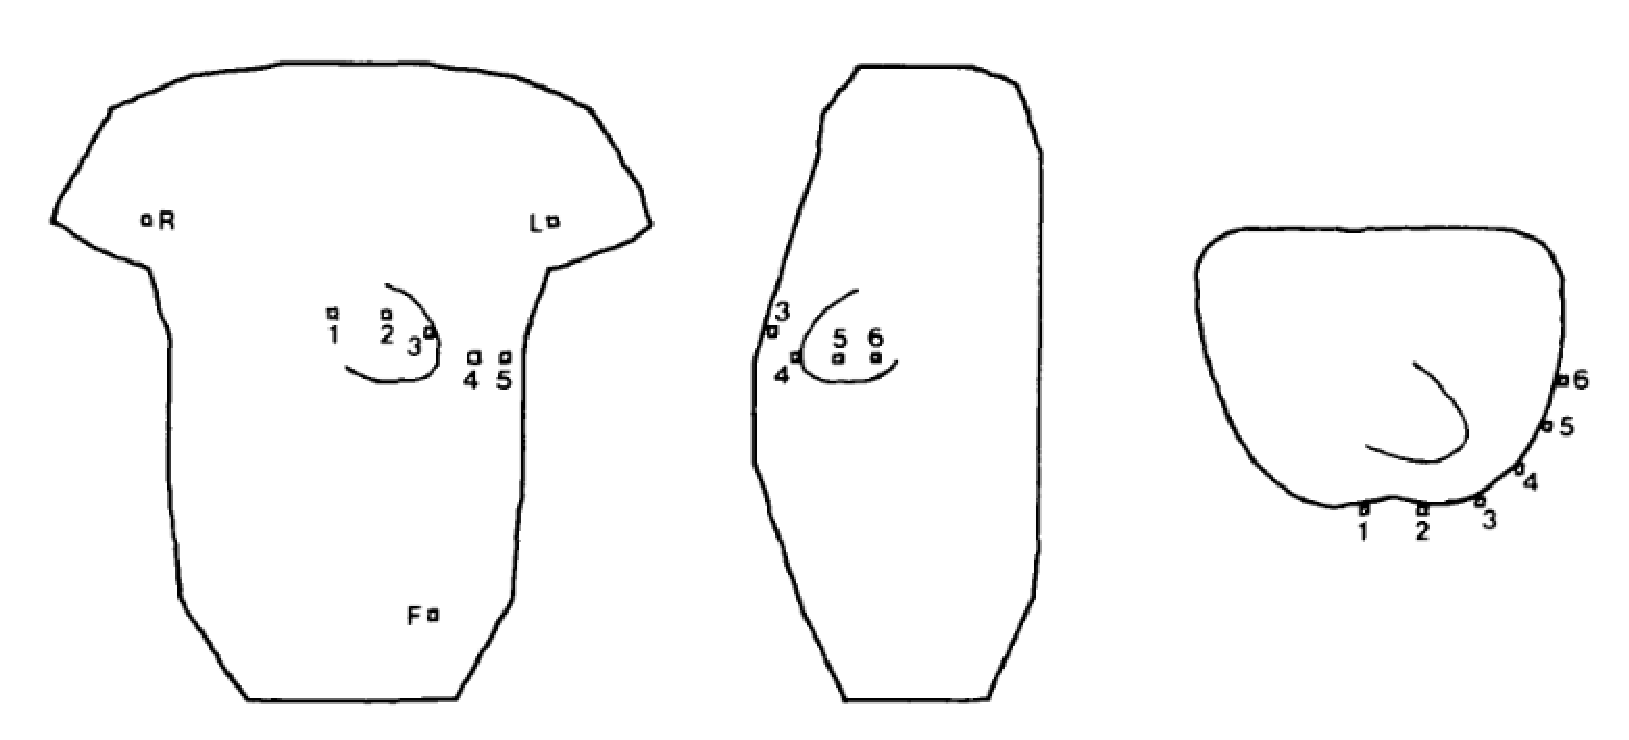
\includegraphics[height=5cm,
    angle=0]{./images/cardiac_torso_Miller1978.eps}}
  \caption{The heart was put in the torso so that the base-apex axis of the
  ventricles was 60$^\circ$ left of front and 35$^\circ$ below the horizontal
  plane. The numbers indicate the location of 12-lead ECG}
  \label{fig:cardiac_torso_Miller1978}
\end{figure}

If the gradient of intracellular potentials exist, then it's assumed that the 
net current flows in the intracellular network from regions of high
intracellular potential to regions of lower intracellular potential is defined
by
\begin{equation}
J_i = -\sigma_i \nabla \Phi_i
\end{equation}
with $\sigma_i$ is the effective conductivity of the intracellular network,
$\Phi_i$ is the intracellular potential. The net intracellular current
density $J_i$ can be interpreted as the current dipole moment per unit
volume in the extracellular medium which is proportional to the spatial
gradient of this intracellular potential distribution. So at first we need to
calculate the voltage gradient $\nabla \Phi_i$, then we estimate the spatial
distribution of $J_i$ as the boundary value problem using $J_i$ as the source of
the volume conductor fields.

To simulate the activation sequences, the isochrones are constructed in 10ms
steps.


\section{Continuum models}
\label{sec:continuous-models}

At the cellular scale, there is a delay between AP of a myocyte and its
neighbors that has been attributed to the effect of gap junctions. This is the
evidence that AP is a discrete process \citep{kleber2004bmc}. However, at a
larger spatial scale, depolarization appears to propagate smoothly
\citep{durrer1970}. 
At large-scale model, a common assumption is that the discrete nature of cardiac
propagation can be neglected, and propagation can be considered as continuous.
This leads to the simplified model approach: monodomain models and bidomain
models. 

Support for this assumption was tested in cultured neonatal rat
ventricular cells.  In 1D strands of a single-cell thickness, the delay by
gap-junctions is about $118\mus$ which is about half of the conduction time
(i.e. significant). However, in strands with several cell layers, the delay was
smaller and amounted to only 20\% of the total conduction time \citep{fast1993}. 

\subsection{Bidomain models}
\label{sec:bidomain-models}

The intracellular and extracellular networks can be
approximated by two parallel continuous mediums with effective conductivities
$\sigma_i$ and $\sigma_e$. The electrical behavior of the resulting continuous
system is described by 2 equations
\begin{equation}
\begin{split}
\nabla \cdot \sigma_i \nabla \Phi_i = I_m  \\
\nabla \cdot \sigma_e \nabla \Phi_e = -I_m
\end{split}
\end{equation}
and $I_m$ is the net trans-membrane current per unit volume (from intracellular
to extracellular medium) [$\muA$/cm$^3$]. If we combine the two above
\begin{equation}
\nabla^2 \Phi_e =- \frac{\sigma_i}{\sigma_e} \nabla^2 \Phi_i 
\end{equation}


As it's imposible to write and solve equations that take into account the
fine-structure details of geometry of the extracellular space and intracellular
space; the microstructure can be averaged (homogenized) to yield equations that
describe the potentials in an averaged, smoothed, and are adequate for most
situations. The bidomain models of cardiac tissue is based on current flow,
distribution of electrical potential, under the assumption of the conservation
of charge andc current \citep{henriquez1993}.

So, at each point in space, it's composed of a certain fraction of intracellular
space and a fraction of extracellular space. Accordingly, each point in space
have two electrical potentials $\phi_i$ and $\phi_e$ (in Volt), as well as two
currents density $\mathbf{J}_i$ and $\mathbf{J}_e$ (A/m$^2$). So, at each point, the relationship
between current and potential follow Ohm-law
\begin{equation}
\mathbf{J}_i = -\sigma_i \nabla \phi_i	\;\;\;;\;\; \mathbf{J}_e=-\sigma_e \nabla \phi_e
\end{equation}
with $\sigma_i, \sigma_e$ are conductivity tensors (S/m). The electric field
$\mathbf{E}$ is
\begin{equation}
\mathbf{E} = -\nabla V_m
\end{equation}

\begin{framed}
What is {\bf conductivity tensor}? - Some materials are anisotropic, e.g. the
heart wall, i.e. they have different properties at different directions. So,
when writing equation for the current conduction, it's not generally valid to
write the scalar $J=\sigma E$, but should write in matrix form
$\mathbf{J}=\sigma \mathbf{E}$, with the conductivity $\sigma$ is rank-2 tensor,
i.e. a 3x3 matrix. So, the component form is $J_i=\sigma_{ij}E_j$.
\end{framed}

When the charges $\mathbf{E}$ are not isolated points, but form a continuous
distribution with local charge density $\rho$, then the flux of charge is called
the {\it divergence equation}. At any time in space, the total current of a
given point is $\mathbf{J}_t=\mathbf{J}_i+\mathbf{J}_e$ and is conserved, unless
there are extraneous current sources, so that $\nabla \mathbf{J}_t=0$.
\begin{equation}
\nabla \mathbf{J}_i = -I_m \;\;\;; \nabla \mathbf{J}_e = I_m
\end{equation}
with $I_m$ (A/m$^3$) is transmembrane current per unit volume (with the positive
axis is pointing outward). The transmembrane current is the current that leave the intracellular space, and
enter the extracellular space, with $I_m$ is composed of a capacitive component
(A/m$^2$) and ionic components (A/m$^2$), including the stimulus current
\begin{equation}
I_m = \chi \left( \Csc \frac{dV_m}{dt} + I_\ion \right)
\end{equation}
with $\chi$ is the surface-to-volume ratio of a cardiac cell, $\Csc$
(F/m$^2$) is the specific membrane capacitance, $V_m$ is the transmembrane
potential.

As $V_m=\phi_i-\phi_e$, then $\nabla V_m=\nabla \phi_i - \nabla \phi_e$, or
$\nabla \phi_i = \nabla V_m + \nabla \phi_e$. So
\begin{equation}
% I_m = \nabla \left( \sigma_i \nabla \phi_i \right) = - \nabla \left( \sigma_e
%   \nabla \phi_e \right)
\begin{split}
I_m = \chi \left( \Csc\frac{\partial V_m}{\partial t} + I_\ion \right) =
\nabla\cdot\left(\sigma_i\nabla V_m + \nabla \phi_e \right) \\
\nabla \cdot \left( \sigma_i (\nabla V_m + \nabla \phi_e) \right) =
- \nabla\cdot\left( \sigma_e \nabla \phi_e \right)
\end{split}
\end{equation}
or 
\begin{equation}
\label{eq:bidomain}
\begin{split}
\chi \left( \Csc\frac{\partial V_m}{\partial t} + I_\ion \right) &=
\nabla\cdot\left(\sigma_i\nabla V_m + \nabla \phi_e \right) \\
\nabla \cdot \left( \sigma_i \nabla V_m \right) &=
- \nabla\cdot\left( \nabla (\sigma_e + \sigma_i) \phi_e \right)
\end{split}
\end{equation}
The two equations of above form the so-called {\bf Bidomain models}.

Under the assumption that there is no electric current flowing from the
extracellular space to adacent spaces, the homogeneous Neuman (no-flus) boundary
conditions can be represented as $\Gamma$:
\begin{equation}
%\begin{split}
\begin{array}{crl}
\Gamma: & \vec{\mathbf{n}}\cdot (\sigma_i \nabla \phi_i) = \vec{\mathbf{n}}
\cdot \left(\sigma_i \nabla (V_m + \phi_e) \right) &= 0 \\
\Gamma: & \vec{\mathbf{n}}\cdot (\sigma_e \phi_e)  &= 0 
\end{array}
%\end{split}
\end{equation}

% At any time in space, the total current of a given point is
% $\mathbf{J}_t=\mathbf{J}_i+\mathbf{J}_e$ and is conserved, unless there are 
% extraneous current sources, so that $\nabla \mathbf{J}_t=0$.
% \begin{equation}
% \label{eq:i_t_conserve}
% \nabla \left( -\sigma_i \nabla \phi_i	+ \sigma_e \nabla \phi_e \right) = 0
% \end{equation}
% The transmembrane current is the current that leave the intracellular space, and
% enter the extracellular space, i.e.
% \begin{equation}
% i_m = \nabla \left( \sigma_i \nabla \phi_i \right) = - \nabla \left( \sigma_e
% \nabla \phi_e \right)
% \end{equation}
% which is the sum of the ionic currents and the capacitive current (including
% the stimulus current), in the case of a biological membrane
% \begin{equation}
% \label{eq:i_m}
% i_m = \chi \left( \Csc\frac{\partial V_m}{\partial t} + I_\ion \right) =
% \nabla\cdot\left(\sigma_i\nabla \phi_i \right)
% \end{equation}
% with $\chi$ is the membrane surface-to-volume ratio which is required to
% convert the current from transmembrane current per unit area to transmembrane
% current per unit volume. The two equations of eq.\ref{eq:i_m} and
% eq.\ref{eq:i_t_conserve} form the so-called {\bf Bidomain models}.


As you can see, the idea of cable theory (Sect.\ref{sec:model-cell})
is extended to higher dimensions to model the complexity of cardiac
microstructure in terms of muscle fibers that branch and anastomose in the
bidomain equations The idea was first proposed by Schmitt \citep{schmitt1969},
and then was formulated mathematically by ~\citep{tung1978}.

Bidomain model is distinct from mono-domain model in that it
made a distinguish between the current flow in the extracellular space
and intracellular space. A bidomain framework define a model of cardiac tissue
that consists of 2 domains: one represents the intracellular domain (subcript
$i$) and one represents the extracellular domain (subscript $e$). A third region
may be included in the bidomain framework, that is called {\it extramyocardial
region} (subscript $o$). The extramyocardial region may represents the fluid
bath (to imitate expeiment conditions), or a torso. \textcolor{red}{It's
assumed that there is no direct currennt flow between the intracellular and
extramyocardial domains}. 


{\bf Boundary condition}: it's typically assumed that there is no current across
the boundary, i.e. no current enter directly into the intracellular space. If
there is an injected current, it enters the tissue through the extracellular
domain, or in the case of extramyocardial domain, through the extramyocardial
domain. In normal condition, extramyocardial draw the current from the
extracellular domain; but in some testing situation, this can be reversed, e.g.
when a defibrillation shock is applied. The three generic variables for each
domain are
\begin{verbatim}
J = current density
Phi = electrical potential
sigma  = conductivity tensor
\end{verbatim}
The transmembrane potential is $V_m=\phi_i-\phi_e$. This is the same as the
definition for a single cell model, except that now the membrane separate
$\phi_i	$ and $\phi_e$ at all points in the cardiac domain $H$.

\begin{framed}
Some researh name the extramyocardial region as extracellular region; while the
extracellular region here is called the interstitial region
\citep{henriquez1990}.
\end{framed}

With a bi-domain structure, the Ohm's law and charge conversion can be modified
to account for the presence of another domain, and boundary conditions must be
altered. The bidomain equation can be derived in several ways, depending on
which dependent variables are required. \citep{keener1998} proposed a practical
algorithm for calculating bidomain electrophysiology.


The defibrillation shock is incorporated into the model as an
extracellular injection of current, or an external applied electric
field in the extracellular domain. The external field is incorporated
through boundary condition on the extracellular potential $u_o$, like
attaching the defibrillation electrodes to the body.

\subsection{Monodomain model}
\label{sec:cont-monod-model}

The early model of the heart consider the conduction along a
representative fibre that was continuous and cylindrical. The approach, known
as {\bf monodomain model}, is is a simplification of the bidomain system
(Sect.\ref{sec:bidomain-models}) where the extracellular domain is 
% assumed to be of highly conducting
% ($\sigma_e=\infty$) or the domains are 
assumed to be equally anisotropic
($\sigma_i = k\sigma_e$).
\begin{equation}
\nabla \cdot (\sigma\nabla V_m) = \chi \left(\Cm \frac{\partial
V_m}{\partial t} + I_\ion \right) 
\end{equation}
with $\sigma = \sigma_i \frac{k}{1+k}$ is the effective conductivity. The
equation is a simplification of eq.\ref{eq:bidomain}. An equivalent form of the
monodomain equation is 
\begin{equation}
\frac{\partial V_m}{\partial t} = \nabla\cdot D\nabla V_m - \frac{I_\ion}{\Csc}
\end{equation}
with $\mathbf{D}=\frac{\mathbf{\sigma}}{\chi}$ (m$^2$/s) is a diffusion tensor
or scalar diffusion coefficient. 



% with the transmembrane potential $V_m=\phi_i$ now (the transmembrane potential
% = intracellular potential). 

With no-flux boundary condition:
\begin{equation}
\Gamma: \vec{\mathbf{n}} \cdot \left( \mathbf{\sigma} \nabla V_m \right) = 0
\end{equation}


The assumptions are:
\begin{enumerate}
\item discrete cellular structures was homogenized into a uniformly
  continuous region, i.e. there is no differentiation between
  cells. 

\item only 1-D and unidirection propagation was considered.
\end{enumerate}
Are these assumptions valid? - it was supported by the experiments of
Weidmann, Chapman and Fry, i.e. cardiac tissues exhibited a syncytial
electrical behavior.



 
\subsection{Monodomain vs. Bidomain}

If there is no injection of current into the extracellular space, the action
potential propagation provided by monodomain 

\subsection{Numerical solution}

Due to the sharp rise in the AP, time steps of around 0.01ms are typically used
to accurately solve the equations using in $I_\ion$. Also, the spatial extent
of tissue undergoing the rapid depolarization is fairly narrow, i.e. the number
of cells having the AP upstroke almost at the same time is faily small; thus, a
small spatial scales is required, e.g. 0.2mm \citep{lines2003}.

Papers: \citep{henriquez1990, henriquez1993, muzikant1998, huang1999,
henriquez2009bidomain}.


\section{Tissue structure: Fiber orientation}
\label{sec:fiber_orientation}


Cardiac tissue is comprised of cells connected by gap junctions, along with
collagen and extracellular fluids. The arrangement of fibers and collagen in the
tissue matrix (extracellular matrix: ECM) is complicated.  Cardiac fibroblasts
plays a major role in maintaining ECM, which provides a framework for cardiac
tissue. Fibroblasts can develop into myofibroblasts, both of which are involved
in the development of fibrosis in the injured heart, and serves as a mediators
of inflammatory responses.

\subsection{Microstructure-based coordinate system}
 
Microstructure-based coordinate system is widely used to model the tissue and
whole-organ. A few hundred years ago (16-th century), it was believed that the
ventricular wall has separate overlapping layers (like layers of the onions),
the outer layer swift each layer consisted of differently directed muscle
fibers. Later on (19-th century), it was accepted that the heart has 4 groups
of fibers: two groups of fibers wind around the outside of both ventricles and
the third one beneath that winds around both ventricles; and the fourth group
winds around only the left ventricle, Fig.\ref{fig:fiber_anatomy}.

\begin{figure}[hbt]
  \centerline{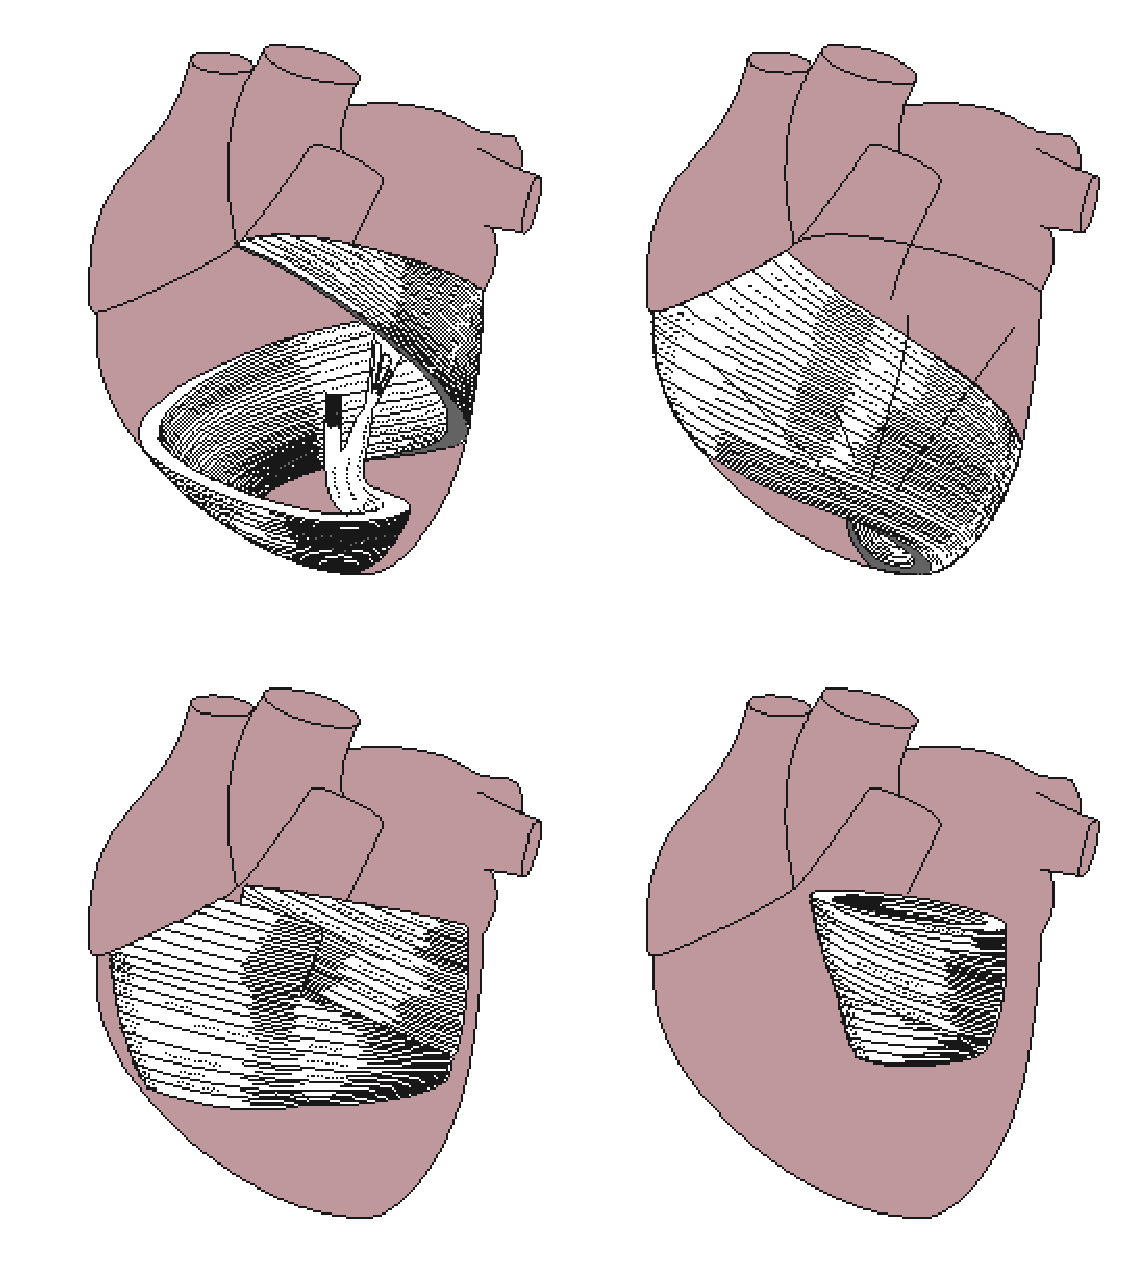
\includegraphics[height=7cm,
    angle=0]{./images/fiber_anatomy.eps}}
  \caption{Orientation of cardiac muscles}
  \label{fig:fiber_anatomy}
\end{figure}

The outter wall is composed of tightly helical, rather than horizontal layers
and the inner wall is composed of looser helix coursing to the apex
\citep{Grant1965}. The apex is probably the oldest part of the left ventricular
muscle embryologically.
For several decades, it was accepted that the ventricles are made up of nested
muscle bundles, each characterized by a well-defined helical fiber path running
from ventricular apex to base. However, ventricular myocardium is now widely
viewed as a continuous structure in which muscle fibers orientation varies
smoothly through ventricular wall \citep{LeGrice1995}. Nevertheless, there is
still convincing evidence for the existence  of discontinuity in myocardial
micro- and macro- architectures. This discrete organization serves an important
mechanical role.

\citep{LeGrice1995} observed laminated appearance of myocardium that resembled
an array of stacked layers or sheets which run in an approximately radial
direction. The circumferential and tangential muscle branches between adjacent
layers is relatively sparse, and the distance between any sheet between two such
branches is 1-2mm. Each sheet consists a tighly packed groups of cardiac
myocytes aligned so that the major cell axis (longitudinal direction of the
cell) is approximately parallel to the cut edge of the layer. At the sheet
level, the layer appears to be uniform in structure. Typically, there are 4
myocytes across the thickness of each layer, with branches between 2 adjacent
layers are generally 1 to 2 myocytes thick.
 
\begin{framed}
Isotropic vs. Anisotropic:

The assumption of transversely isotropic means the propagation speed depends on
muscle fiber orientation, but is independent of direction in the plane
transverse to the muscle fiber axis.
\end{framed}
 
In the heart, the usual directions are longitudinal, transmural and
circuferential, i.e. (L,T,C) system, Fig.\ref{fig:cardiac_coordinate}. In
systole, there is longitudinal shortening, transmural thickening, and
circuferential shortening. Previously, to study 3D morphology of cardiac collagen structures,
\citep{dolber1993} stained collagent with picrosirius red (PSR) which is a
specific stain for collagen type I, II and III.
This allows optical sectioins to be imaged up to 10$\mum$ deep into the tissue
with acceptable signal-to-noise ratio. However, this is not enough due to a
typical muscle layer is 50$\mum$.

To know detail 3D structure, \citep{Young1998} used
confocal microscopy to image a serial of images at different depths via optical
sections. The wedge they used is of size 3800$\times 800\times 800 \mum^3$ in
volume, with a voxel size is 1.56$\mum^3$. This allowed them to examine
distribution and morphology of myofibres, collagen, extracellular matrix and
major vessels within the wedge. Pixels as collagen were linearly mapped to
grey-scale  range 128-255, pixels labelled blackground are in the range 0-29;
and those were neither collagen nor background were labelled myocytes and mapped
to the grey-scale in the range 30-127.

\begin{figure}[hbt]
  \centerline{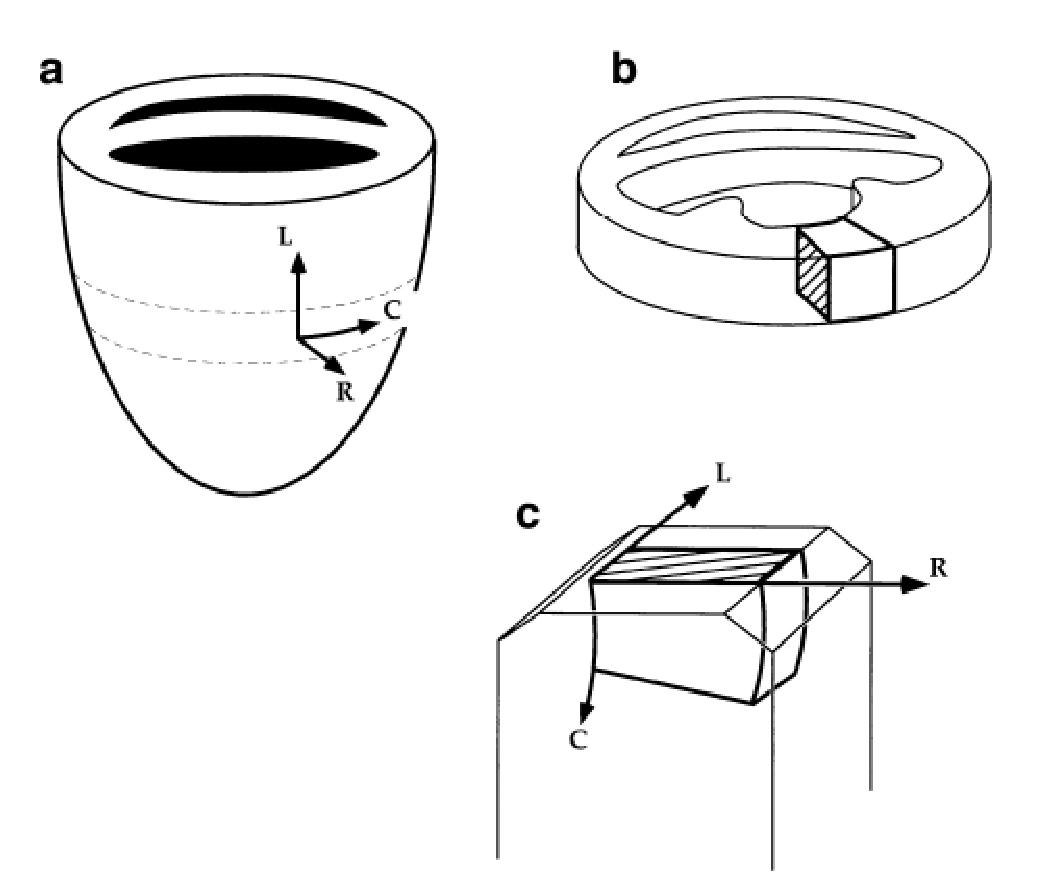
\includegraphics[height=5cm,
    angle=0]{./images/cardiac_coordinate.eps}},
      \centerline{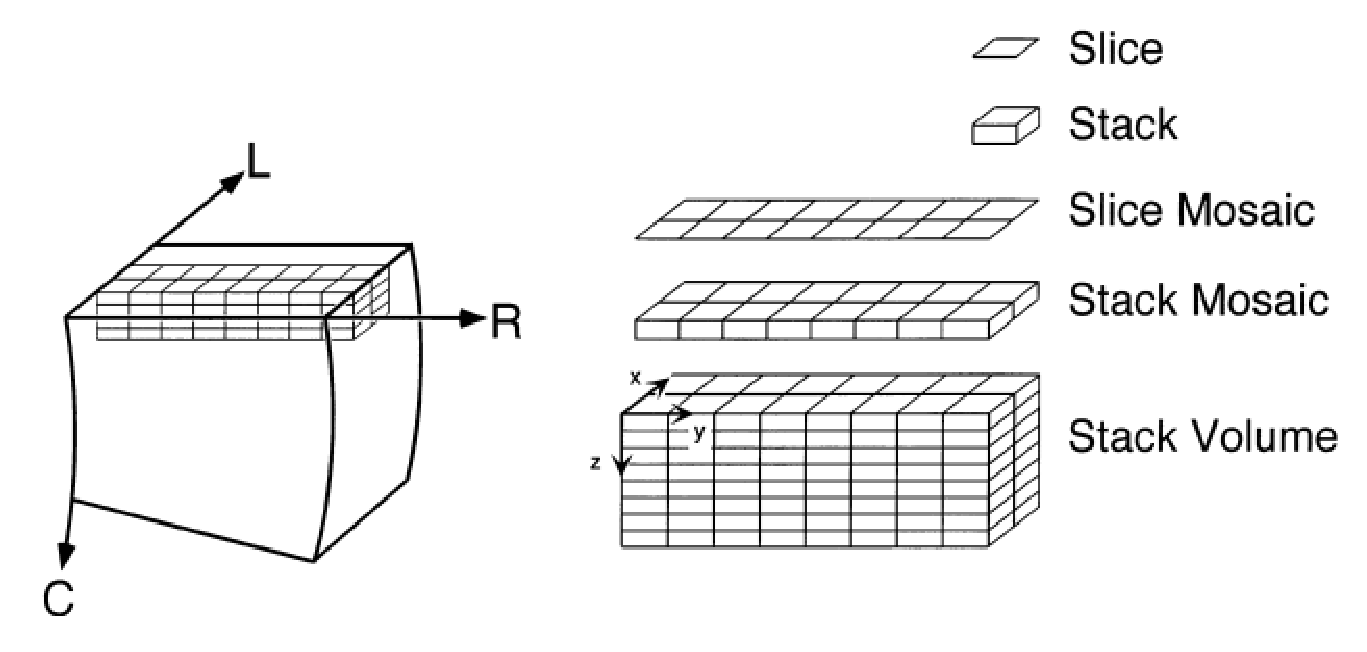
\includegraphics[height=5cm,
    angle=0]{./images/cardiac_segments.eps}}    
  \caption{(A) Cardiac coordinate system (L,T,C) (a) an equatorial ring of 2mm
  thick is removed from the heart; then from this, a transmural segment of LV
  free-wall of $\approx$ 2mm wide was cut out.
  (B) The volume is assembled from an array of contiguous image stacks, each consists of 40 image slices
  (optical sections). (x,y,z) is the image-coordinate system}
  \label{fig:cardiac_coordinate}
\end{figure}

The images were captured in the circumferential-longitudinal (C-L) aspect; then
the tissue block was then rotated 90$^\circ$ and imaged in the
circumferential-radial (C-R) plane. The stacks of images in the C-R plane were
then digitally resliced in the C-L plane, allowing comparison of the dimension
of structures imaged in the two orthogonal planes. Here, a 'slice' denotes a
single optical section, a 'stack' is a single 3D acquisition of 40 optical
sections; a 'slice mosaic' is a set of slices at the same z-location (or
lateral plane) and 'stack mosaic' is a set of stacks obtained from the same
z-location. Finally, a 'stack volume' is the extended 3D image data set built
upon the set of stack mosaics.
 

The axes of this coordinate system are defined as follows. Given that the
laminated sheet structure of endocardial fiber, a orientation of the cardiac
cells in each layer gives the first microstructural axis, i.e. (local) {\bf
fibre axis} $\nu_1$. As planar shape of the laminated sheets, the second
microstructural direction is given by the vector $\nu_2$ in the plane of the
sheet that is  perpendicular to the fibre axis. This is called {\bf sheet axis}.
The third axis is calculated through the cross product of the first two axes
creating a third vector that is normal to the plane of the sheet, called {\bf
cross-sheet axis}, $\nu_3$.

\begin{figure}[hbt]
  \centerline{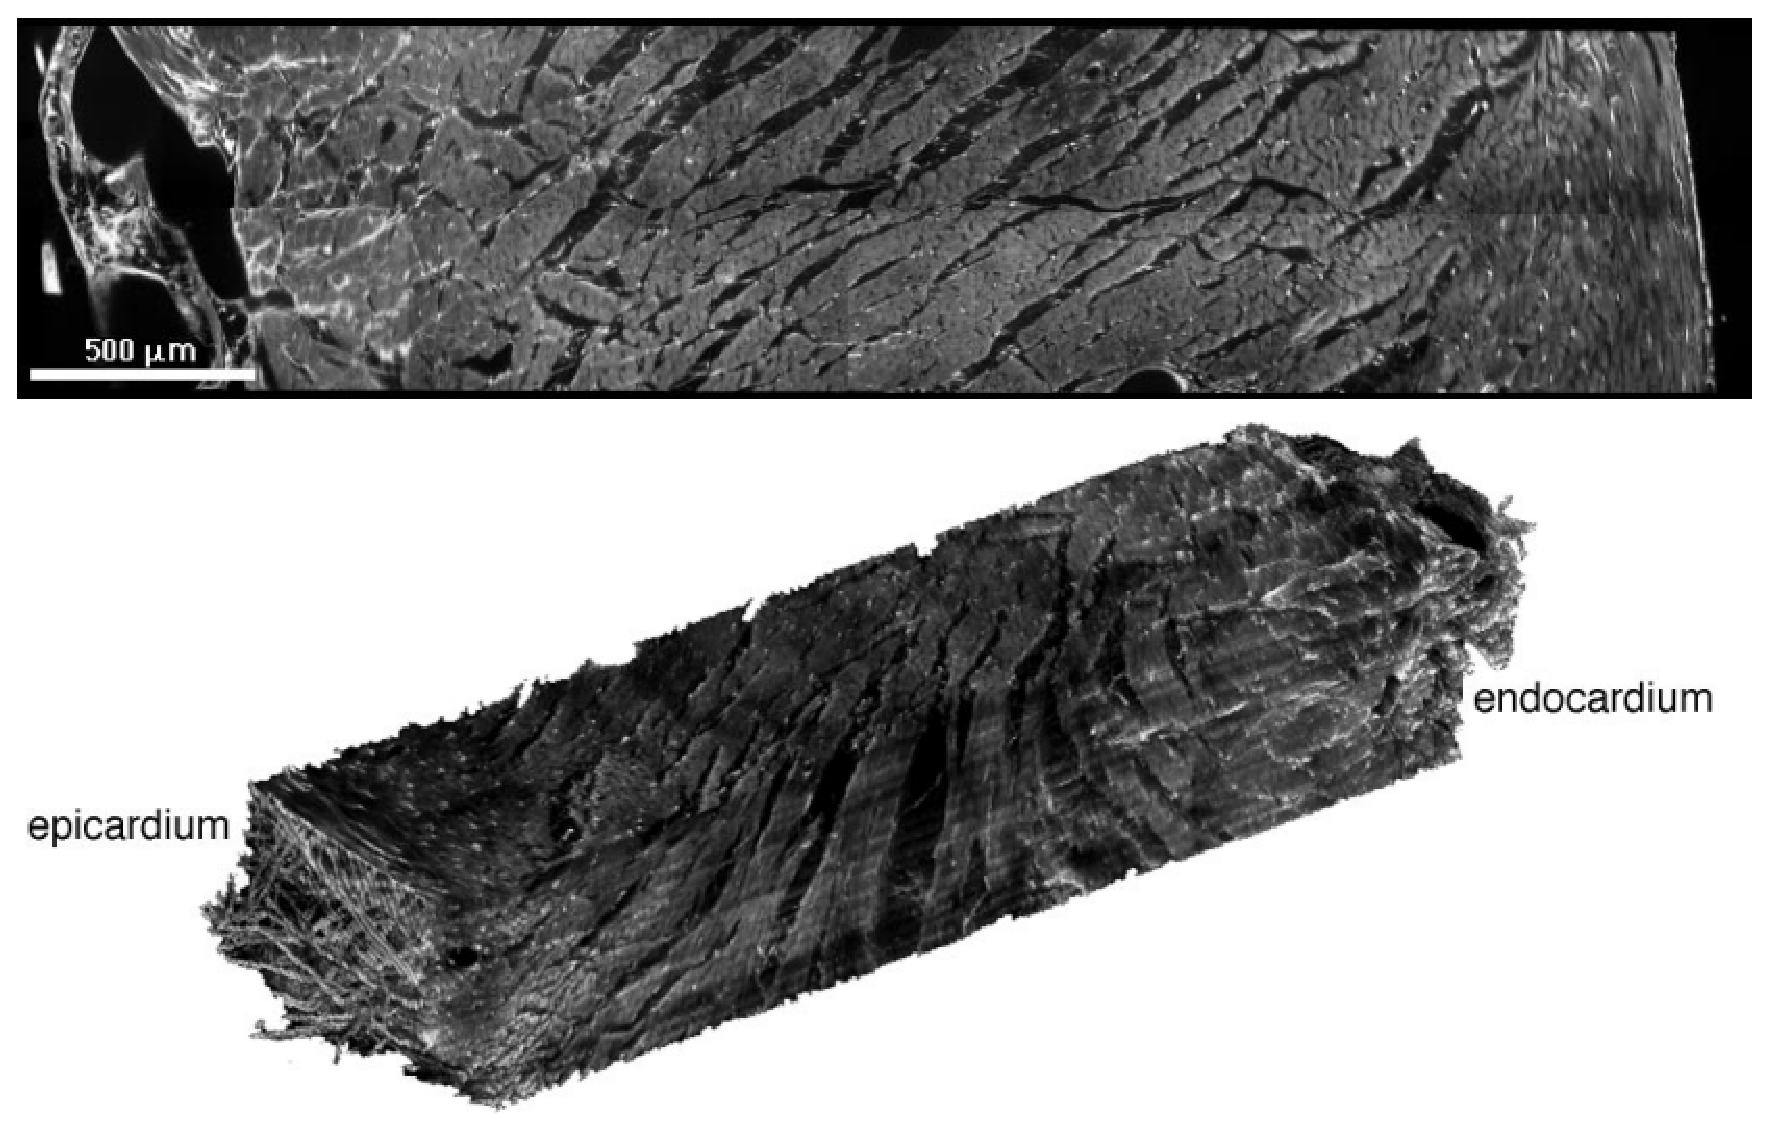
\includegraphics[height=7cm,
    angle=0]{./images/cardiac_slices.eps}}
  \caption{}
  \label{fig:cardiac_slices}
\end{figure}


\subsection{Fiber orientation}

The distribution of stress is not only the function of tension but also the
spatial orientation of the fibers. \citep{Streeter1969} showed that the wall is
characterized by a gradual change in fiber angle from Endo- to Epi- cardium.
Fig.\ref{fig:cut_fiber} (B) demonstrate how a wedge is extracted from the heart,
and the local axes for the wedge (specimen) is defined. NOTE: The origin of the
local coordinate is on the epicardial surface. Then, the fiber angle $\alpha$ is
positive when measured counterclockwise from the local $v$-axis. So, the fiber
angle $\alpha$ is from -90$^\circ$ to +90$^\circ$. IMPORTANT:
\textcolor{red}{The local $w$-axis is not necessarily parallel to the $z$-axis
of the heart}. The extremes of fiber angle tend to approach 90$^\circ$ at the
Endo- and -90$^\circ$ at the Epi-surface.

\begin{figure}[hbt]
  \centerline{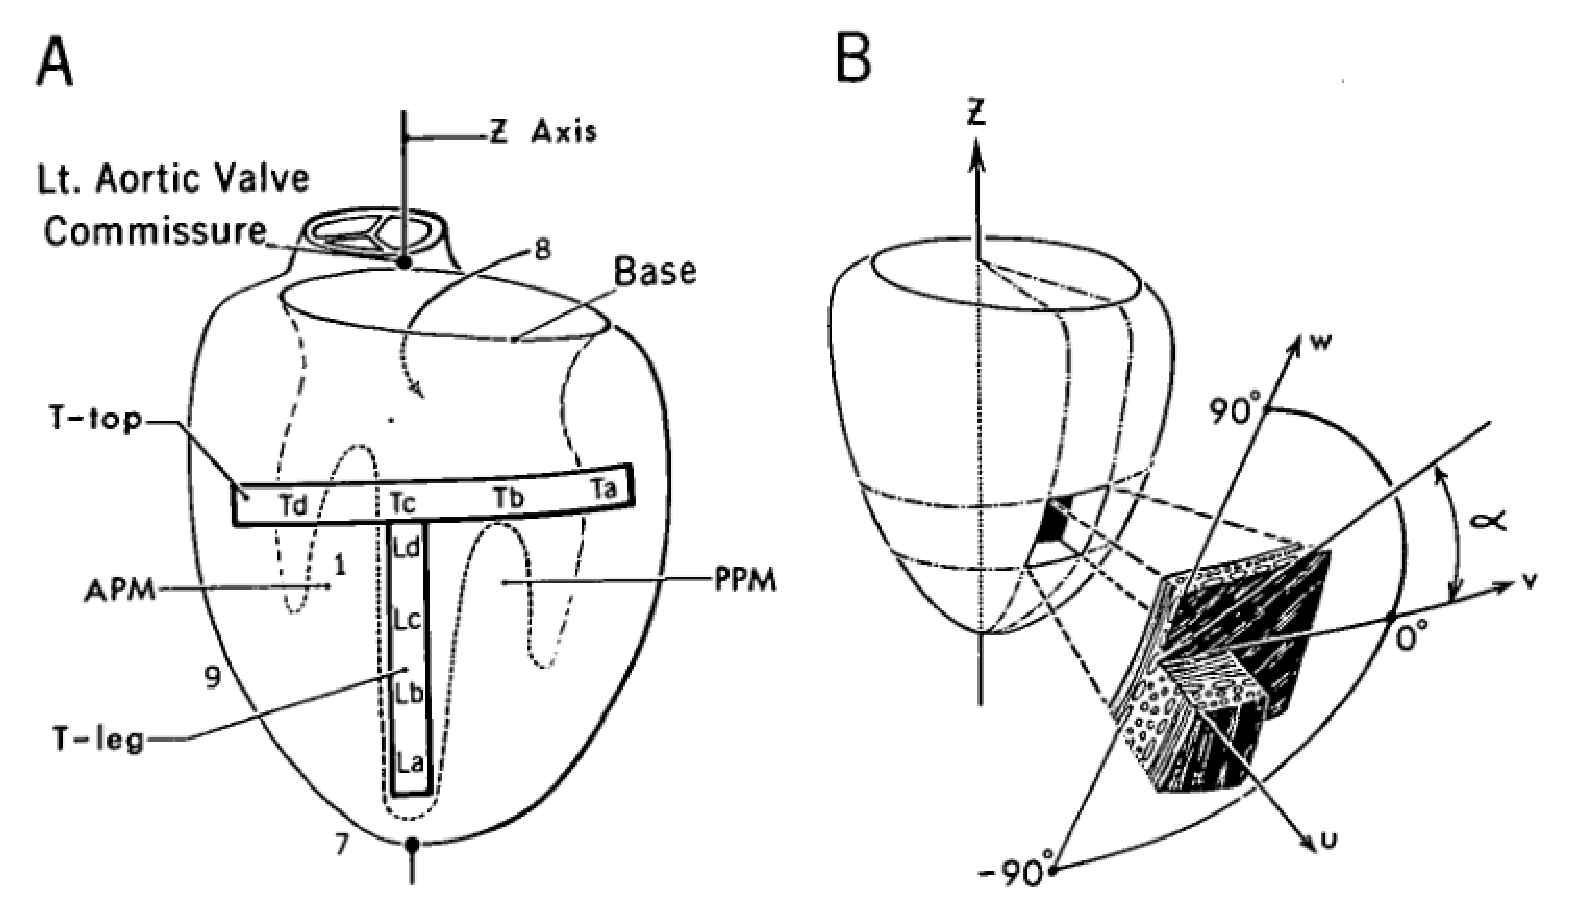
\includegraphics[height=7cm,
    angle=0]{./images/cut_fiber.eps}}
  \caption{(B) a full-thickness specimen is cut out from the wall of the left
  ventricle. Local axes  $u,v,w$ on the specimen are defined by the local
  normal, latitude and longitude, respectively, for a given site on the Epi-
  surface. (A) APM=anterior papilary muscle, PPM=posterior papilary muscle
  \citep{Streeter1969}}
  \label{fig:cut_fiber}
\end{figure}

To determine the fiber orientation at different regions, a T-shape specimen (3mm
wide) is cut out from the heart, Fig.\ref{fig:cut_fiber}(A) show 8 sites on the
T-shape specimen being used for measurement of fiber orientation
(Td, Tc, Tb, Ta, Ld, Lb, Lc, La). The T-top extends from basilar region near,
but excluding the APM root to the posterior demarcation of the right and left
ventricular walls. The leg of T-shape extend from the middle of the T-top (i.e.
between two papillary muscles) to the ventricular apex. Additional sampling
sites are numbered  (1, 7, 8, 9): 1=root of APM, 7 = same meridian of 9 and
almost at the apex and anterior to the root of APM, 8 = on the interventricular
septum, 9 = left-ventricular side. Each location we cut out a block of 8x8mm
through the left-ventricular wall.

The fiber angle changes smoothly across the wall in both systole and diastole,
Fig. \ref{fig:fiber_orientation_systole_diastole}. As you can see, the
transition from diastole to systole correspond to an approximate constant angle
increase through the wall at any sampling sites. This increase is abotu
7$^\circ$ at the T-top and 19$^\circ$ in the T-leg. This difference in the T-leg
compared to T-top can be due to the bending of Z-axis during contraction or the
torsonal rotation. The change in angle w.r.t.
the  wall thickness represented as $d\alpha/dh$ is largest near the endocardial
and epi-cardial surface.

\begin{figure}[hbt]
  \centerline{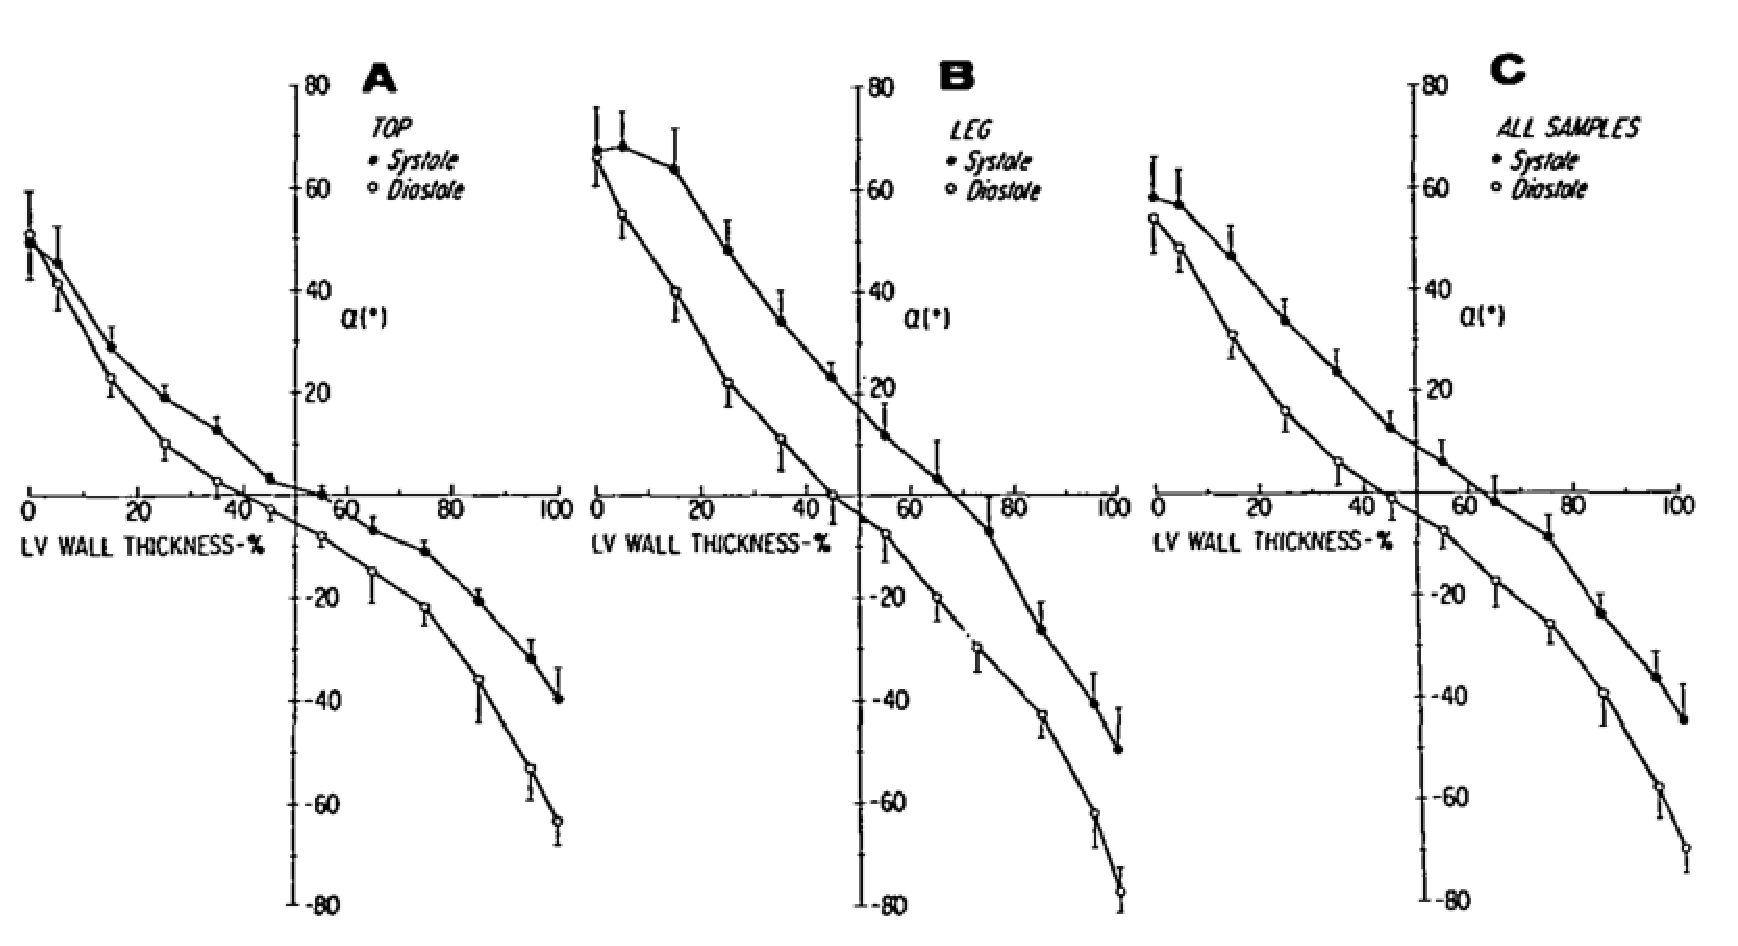
\includegraphics[height=7cm,
    angle=0]{./images/fiber_orientation_systole_diastole.eps}}
  \caption{Averaged data from 5 hearts in systole and diastole. Zero percent of
  wall-thickness implies Endocardial surface.}
  \label{fig:fiber_orientation_systole_diastole}
\end{figure}




\section{Transmurral repolarization gradient in Epi-M--Endo cells}

The distinct regional differences lead to the different AP morphology is shown
in Fig.\ref{fig:AP_morphology}. Each subplot has 6 curves, representing cycle
length (CL) from 300-8000ms [NOTE: basic cycle length (BCL) is normal heart
rate, e.g. BCL=2000ms means heart rate =0.5Hz or 1beat-per-2sec]. The result
shows that M-cells have the longest APD, at slow rates. The transitional cells
(cells 2-5) were isolated from the mid-myocardial region.
The distinction has been observed in canine, feline, rabbit, rat and human
heart. M-cells are thought to contribute 30-40\% of the ventricular wall, and
thus can contribute importantly to the body surface ECG. Transmural dispersion
of repolarization has been shown to play a role in the genesis of VT and VF in
different animal models of heart failure (HF) \citep{glukhov2010}. APD
differences is more prominent in non-failing hearts, while it's more uniform in
failing hearts, Fig.3 \citep{glukhov2010}.

 
\textcolor{blue}{M cells and Epicardial cells, but not endocardial cells,
display APs with a notched and spike-and-dome morphology}. This is the result of
prominent, transient, outward-current $I_\to$ in phase I. M-cells locate in the
deep structures of canine, guinea-pig, rabbit and human ventricles (but not in
rat) \citep{antzelevitch2001}. $I_\to$ is 4-aminopyridine (4-AP) sensitive
transient outward current which is much smaller in endocardium. Also, $I_\to$ is
much larger in the right than in the left ventricular epicardium
\citep{didiego1996}. 

\begin{figure}[hbt]
  \centerline{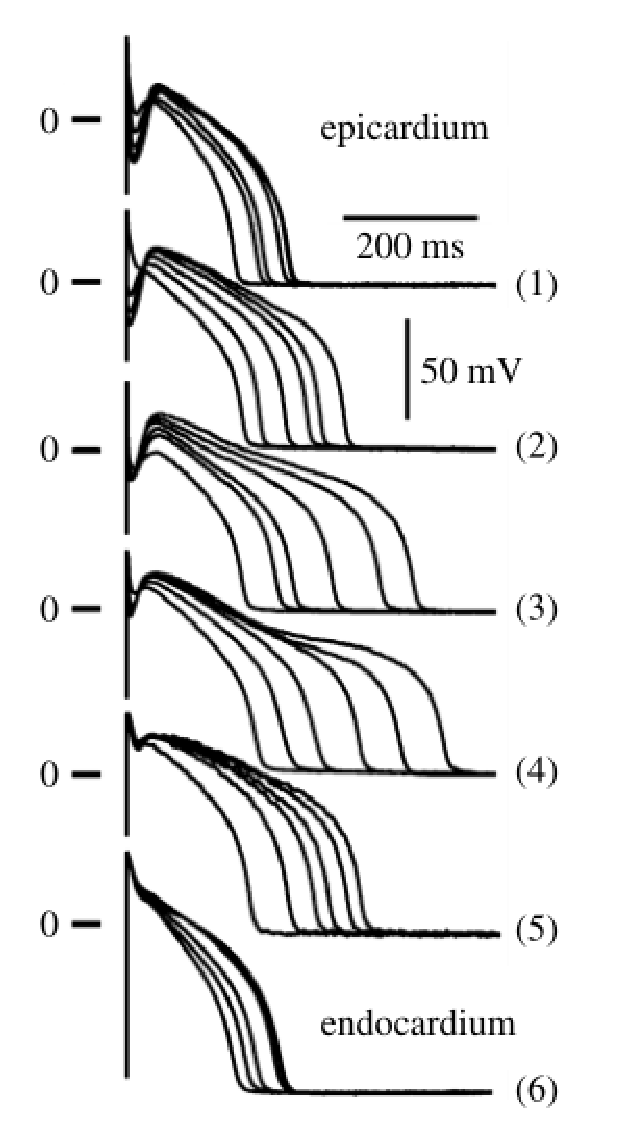
\includegraphics[height=6cm,
    angle=0]{./images/AP_ventricles.eps}}
  \caption{Transmembrane AP recorded from myocytes in Epicardial, M-cells
  (mid-myocardials), and Endocardial cells of canine left ventricles
  \citep{antzelevitch2001}}
\label{fig:AP_morphology}
\end{figure}

The transmural gradient in amplitude of AP  underlies the normal J-wave or
Osborne wave of the ECG. The exaggeration of this transmural gradient has been
linked to the apperance of pathophysiological J-wave, ST-segment elevation and
the development of VT/VF in patients with the Brugada syndrome.

The larger APD in M-cells than in Epicardial and Endocardial cells are due to
the presence of a smaller (slow-activating delayed rectifier) $I_\Ks$
\citep{liu1995}, a large late sodium current (late $I_\na$)  
\cite{antzelevitch1999} and a large NCX current \citep{zygmunt2000}.
\textcolor{red}{NOTE: Wheter late $I_\na$ is a distinct sodium channels or the
late activation of a typical sodium channels is not well understood.}

\begin{framed}
In canine heart, rapidly activating delayed rectifier $I_\Kr$ and
inward-rectifier $I_{\k1}$ are the same, i.e. no transmural differences. 
\end{framed}


M cells have a smaller net repolarizing current make it more sensitive to
APD-prolongation agents than in other cell regions (Epi- and Endo-cardium), e.g.
\begin{enumerate}
  \item $I_\Kr$ blockers like D-sotalol, E-4031, almokalant and erythromycin.
  \item agents that increase $I_\ca$: Bay K 8644
  \item agents that increase late $I_\na$ ($I_{\na,L}$: ATX-II and
  anthopleurin-A
\end{enumerate} 
Exceptions are agents that block $I_\Ks$: azimilide, quinidine, pento-barbital,
amidarone, and chromanol 293B. The situation is more complicated for drugs that
affect more than two channels types, e.g. quinidine, pentobarbital, amiodarone,
and azimilide. NOTE: In the case of quinidine, a low level (3-5$\muM$) can
produce a marked prolongation of M-cell APD, but not in Epi-and Endo-cardium
(as the predominant effect to block $I_\Kr$ at this concentration). At higher
concentration (10-30$\muM$), it blocks both $I_\Ks$ (prolong APD in Epi-and
Endo-cardium) but also block late $I_\na$ in M-cell (that abberviates the
effect of blocking $I_\Ks$ causing a non-change in M-cell APD).

The transmural ECG is recorded using the so-called {\bf wedge preparation} for
left-ventricle, Fig.\ref{fig:wedge_preparation}. The wedge is stimulated from
endocardial surface, so that transmembrane AP is recorded simultaneously from
Epi-, M region (M) and Endo sites using three micro-electrodes. Transmural ECG
is recorded along the same transmural axis, registering the entire field of the
wedge. 

\begin{figure}[hbt]
  \centerline{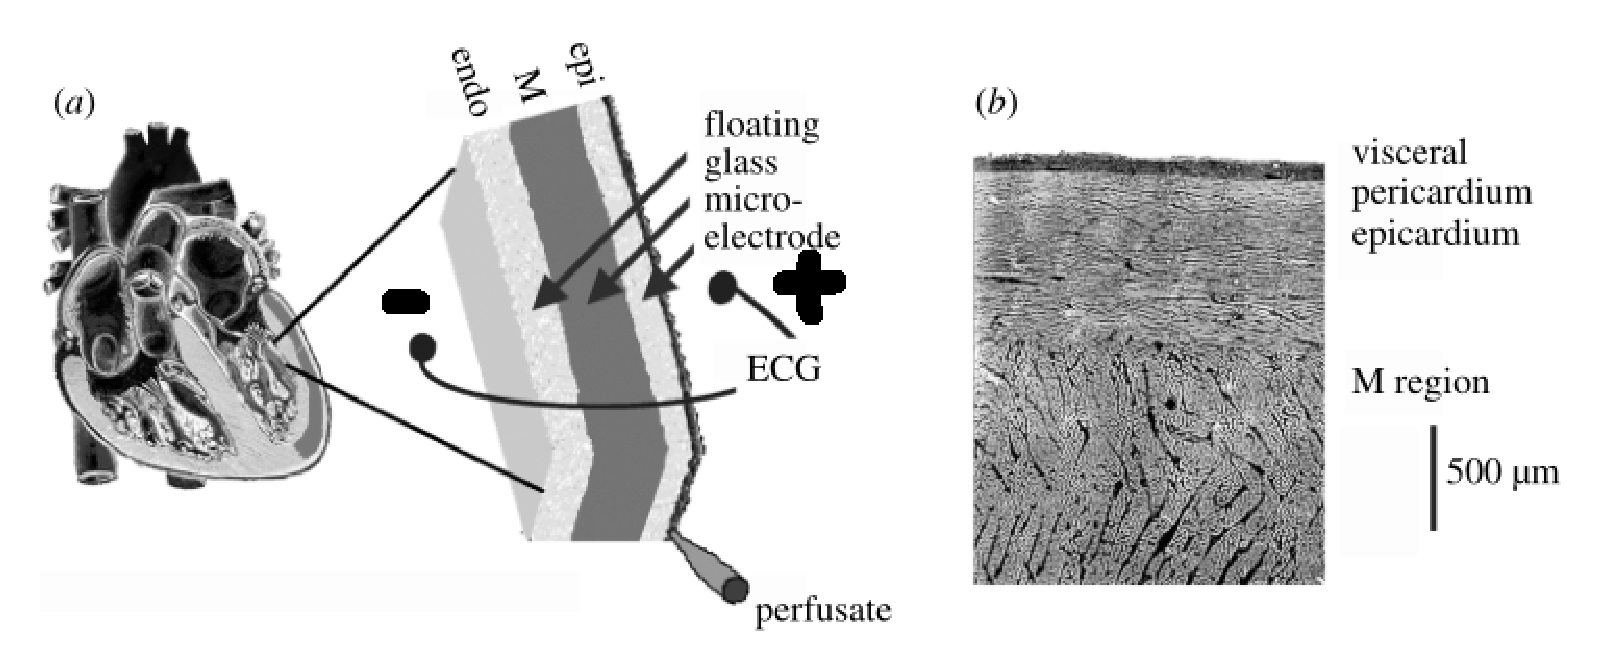
\includegraphics[height=4cm,
    angle=0]{./images/wedge_preparation.eps}}    
\caption{(A) Wedge preparation of canine left ventricle (LV). (B) M-cells
orientation is different that of Epi-cardium}
\label{fig:wedge_preparation}
\end{figure}

Regions of high resistivity match with cell longitudinal orientation, while
regions of smaller resistivity match with the transition of cell orientation to
transmural orientation, Fig.\ref{fig:wedge_preparation}(B) and
Fig.\ref{fig:wedge_APD_resistance} (B). The conduction time (CT) and
repolarization time (RT) is given in Fig.\ref{fig:wedge_APD_resistance}(A) paced
at 0.5Hz. A sharp transition in APD90 occurs between epi- and sub-epicardium.

\begin{figure}[hbt]
  \centerline{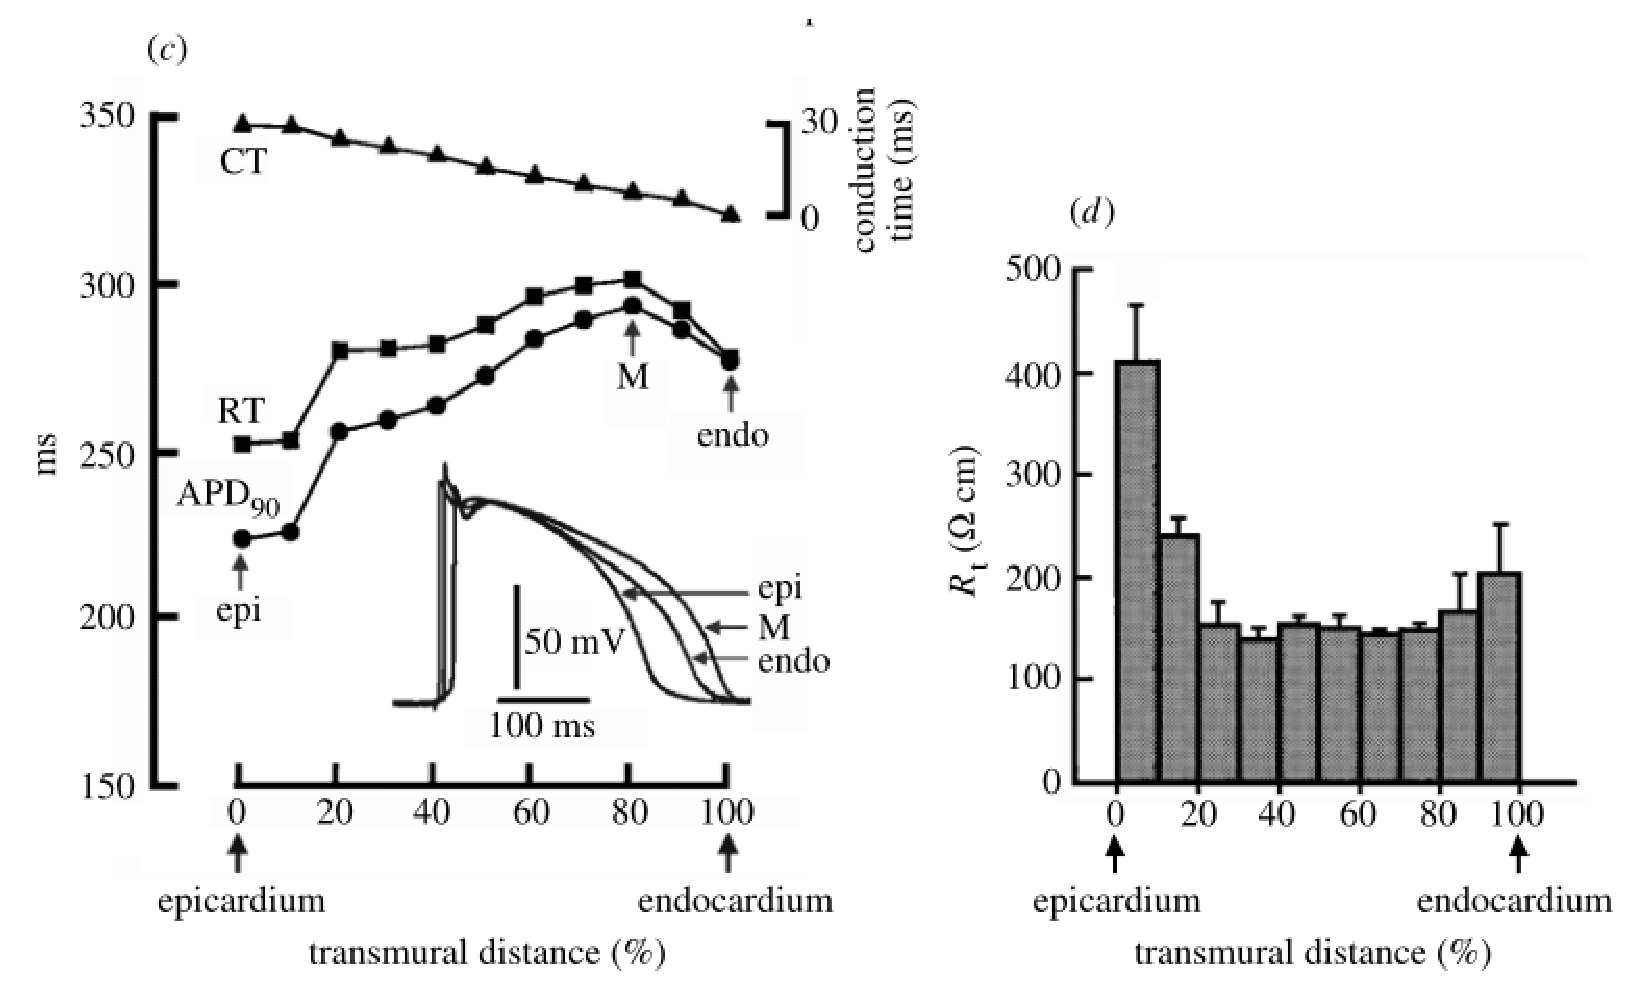
\includegraphics[height=4cm,
    angle=0]{./images/transmural_APD_resistance.eps}}    
\caption{(A) APD90 increase from Epi- to M-cells and then decrease to
Endocardium; RT=APD90 + CT; (B) distribution of total tissue resistivity
($R_t$) across canine left ventricle}
\label{fig:wedge_APD_resistance}
\end{figure}






\section{Electrotonic coupling (cardiac gap junctions)}

The conduction of the electrical signal is dependent on both the active membrane
properties (the action potential) and the passive properties determined by the
architectural features of the myocardium. The transfer of ionic currents between
cardiac cells occurs at {\bf gap junctions} which play a pivotal role for the
velocity and the safety of impulse propagation in cardiac tissues. Under
physiologic conditions, the gap junctions are tightly packed with the rod-shaped
cardiomyocytes giving an anisotropic conduction, which is continuous at the
macroscopic scale. However, at the microscale, using computational simulations,
gap junctions limit the axial current flow and to induce 'saltatory' conduction
at unchanged overall conduction velocities. This discontinuities disappear in 2D
and 3D tissues due to lateral averaging of depolarization current flow at the
activation wavefront \citep{rohr2004prop}.


\citep{hoyt1989} using canine and electron micrographs showed the following
components, Fig.\ref{fig:micrograph_cardiac}
\begin{enumerate}
  \item junctional membrane: a specialized plasma membrane connecting 2 cardiac
  cells
  \item intercalated disc: a subset of junctional membrane containing
  interdigitating processes of adjacent cells
  \item plicate segment: a portion of the intercalated disc containing a
  finger-like interdigitating processes of cell adhesion
  \item interplicate segment: a portion of the intercalated disc
  
  \item gap junction: a specialized region in the intercalated  disc with
  longitudinal extent of the large gap junction is 1.3$\pm$0.8$\mum$, while
  transverse extent was 5.1$\pm$2.0$\mum$ (corresponding to the mean surface
  area of 6.6$\mum^2$). That explain why the coupling in the transversal
  direction between cells are weak.
  
  \item \ldots
\end{enumerate}

The studying of 3-dimensional structure and distribution of intercellular
junctions in cardiac myocytes is important in understanding the patterns of
electrical conduction in myocardium. In ventricular myocardium, large
intercalated discs exist at the end of the myocytes, with smaller discs along
the length of the cell \citep{severs1990}. Averaged intercalated discs in mature
human ventricular cells are 11.6 \citep{peters1993}. 

Gap junctions have integral proteins called {\bf connecxins} in hexameric units
called {\it connexons}, each possesses a 1.5-2.0nm central pore. There are 3
types: connexin40 (Cx40), Cx43 and Cx45. The fourth type of connexin, Cx37, is
only found in endothelial lining \citep{vanVeen2006}. The connexons
in the adjacent cells align to form a complete channel linking the cytoplasic
compartments, providing a relatively low-resistance pathway for ion movements
(molecules upto 1kD) and electrical propagation \citep{imanaga1987, spray1990}.

\begin{figure}[hbt]
  \centerline{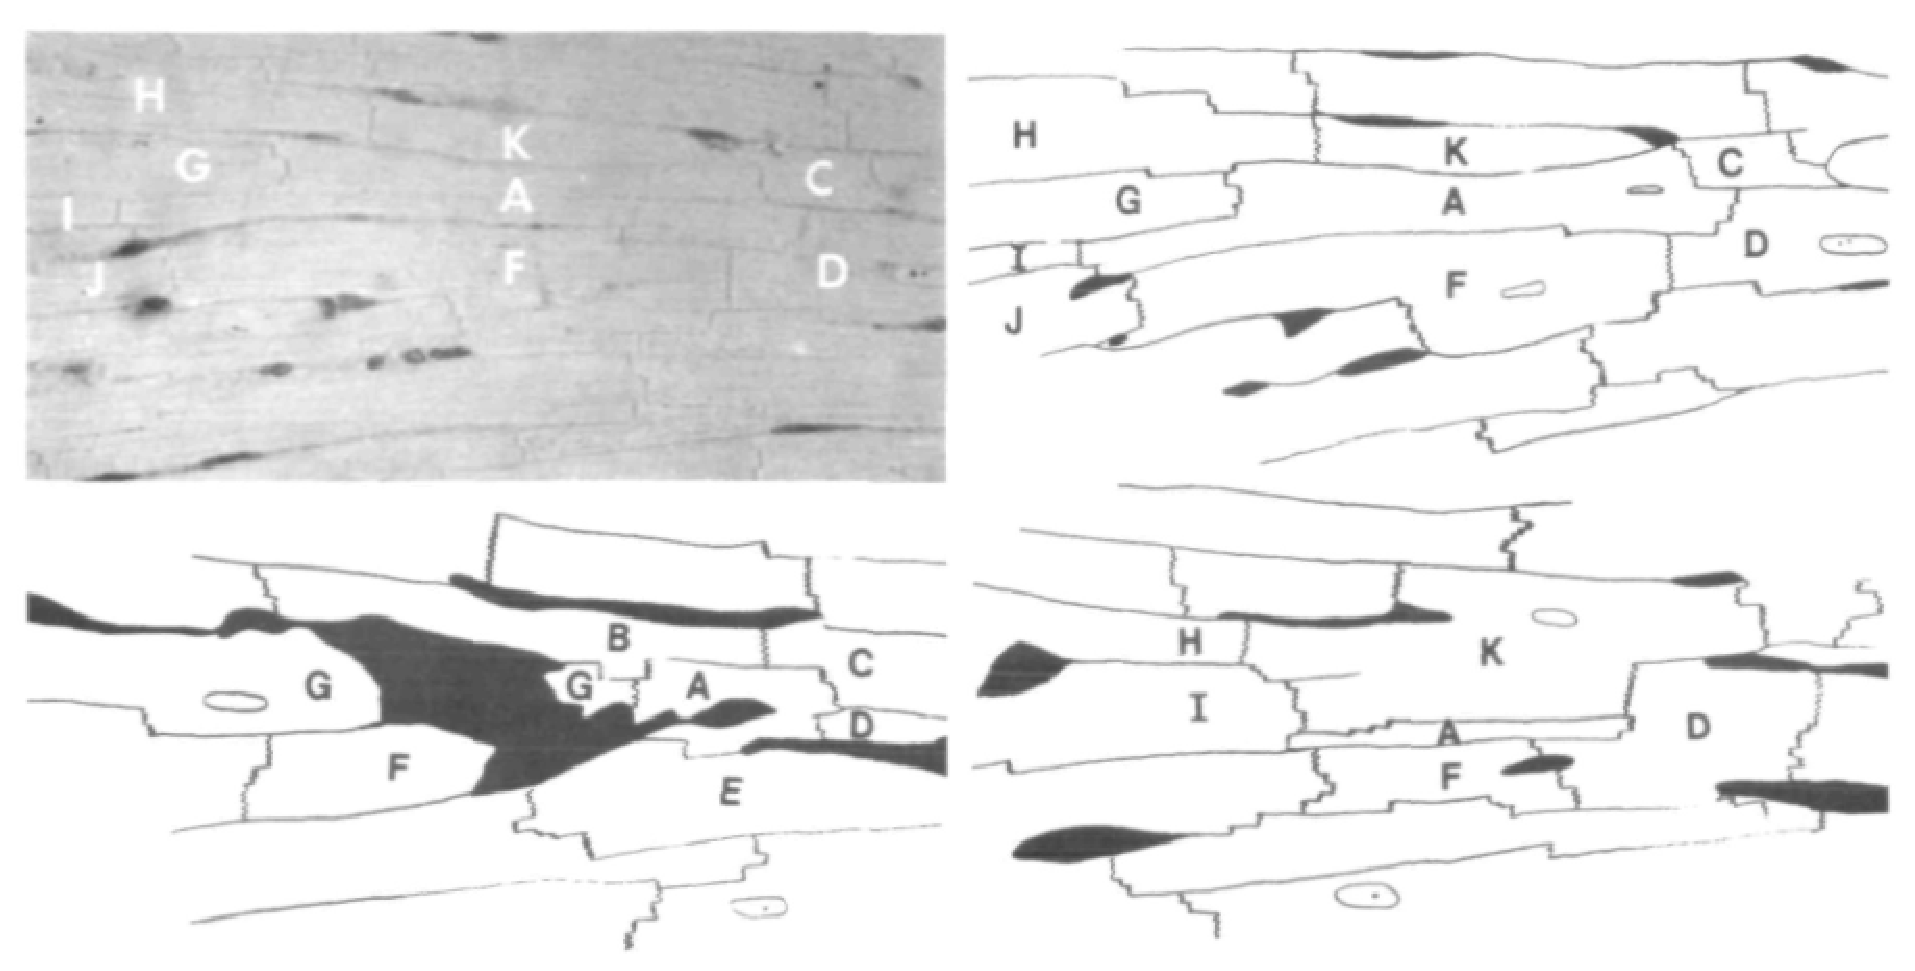
\includegraphics[height=5cm,
    angle=0]{./images/micrograph_cardiac.eps}}
  \caption{(A) Photmicrograph of myocardium; (B,C,D) the drawing showing the
  multiplicity of myocyte interconnected to each other at intercalated discs at
  42 consecutive 2$\mum$ thick plastic sections (shaded areas denote prominent
  interstitial vessels and septae)
  \citep{hoyt1989}}
\label{fig:micrograph_cardiac}
\end{figure}

\begin{framed}
Each gap junction, on microscopy, showed irregular clusters of channels (with
$> 2\mum$ in diameter) and contains upto thousands of connexons. It's important
to know that the coupling between 2 adjacents are not fixed, but depending on
the state of gap-junctional channels, which can be open or closed. The
proportion of channels in open state and the permeability/conductance of each
channel are determined by the connexin isoform composing the channel.

A connexin43 in its main conductance state is on the order of 40pS or 60pS., but
the physiological and pathological significance on the conductance state is
unclear.

A connexin40 in its main conductance state is 150 to 200pS. The abundance
amount of connexin40 at His-Purkinje tissue explain the high conduction velocity
in this region.

A connexin45 in its main conductance state is 22pS to 36pS.
\end{framed}

Using regularly spaced cylinders packed end-to-end and side-to-side is a quite
simplifications in model studies. In deed, the interconnections of cardiac
myocytes are more complex, as cells overlap and not strictly longitudinally or
transversely situated with respect to each other. Distribution:
\begin{enumerate}
  \item \citep{hoyt1989} used morphometric analysis of left ventricular
  myocardium sectioned in 3 orthogonal planes showed that 80\% of gap junctional
  membrane occur in large, ribbon-like gap junctions oriented trasversely at
  cell end processes; only 20\% gap junctional membrane are small gap junctions
  located at plicate segments of intercalated discs (cell-to-cell adhesion). In
  canine, about 34\% of overall cell length has intercalated disc at the cell
  terminal, and 29\% of side-to-side, and the others has combination of both.
  
  \item
\end{enumerate}
So, a  'typical' cell-end may lie in the central portion of the cell body, with
each cell is electrically coupled to an average 9 other myocytes; with 11-12
other muscle cells in canine \citep{hoyt1989}. Using computational models,
\citep{rudy1991} estimated to be 11 adjacent myocytes on average.



So, depending on the local potential gradients, they may determine the ion
movements through gap junctions. Thus, local transverse ion movement could occur
during global longitudinal conduction. However, this transversal coupling can be
lost with aging \citep{spach1986}. Gap-junctional channels create continuity
between cytoplasmic compartments of adjacent myocytes, but act as resistive
discontinuities to the cytoplasmic current flow between intracellular
compartments of the cells. Given the ratio of cell length to width in isolated
canine ventricular myocyte of 6:1, the tissue has fewer cell boundaries per unit
distance in the longitudinal vs. transverse direction; thus the longitudinal
resisitivity is lower. In normal ventricular myocytes, this is about 3.4x more
rapid than in the transverse direction \citep{hoyt1989, saffitz1995}. This
anisotropy is considered uniform, because the advancing wave front is considered
'smooth' \citep{spach1982}. The resistivity of gap-junctional membrane although
several orders lower than non-gap-junctional plasma membrane, it's still several
orders of magnitude higher than cytoplasmic intracellular resistivity.

\begin{framed}

Another complexity is in papillary muscles where the cells are grouped into 2-30
cells (surrounded by connective tissue seath) with strong coupled in both
longitudinal and transversely due to multiple intercellular connections
\citep{sommer1982}. Adjacent unit bundles are connected to each other in a
lateral direction at intervals 100-150$\mum$, which is expected to contribute
further to the anisotropy of conduction. However, its relevant to other regions
of ventricular myocardium is unknown \citep{peters1998}.
\end{framed}

The abnormalities in the conduction of the cardiac impulses are important to the
cause of arrhythmias, in that they alter the path length, conduction velocity,
and recovery of excitability \citep{spach1982, spach1986}.
 

\section{Geometric modelling}
\label{sec:geometric_modelling}

A mathematical and computational representation of the heart that require
anatomical and structural details can be challenging. The standard approach is
to represent the geometry of the solution domain using {\bf blocks} or {\bf
elements}; that, if made small enough, capture required level of detail. The
structure of blocks/elements is known as a {\bf mesh}. Computationally, each
block/element is represented as a set of {\bf nodes} that are often element
vertices. So, each element is a triangle or a tetrahedron. To generate this
mesh, we need some
libraries\footnote{\url{www.robertschneiders.de/meshgeneration/software.html}}
that utilize methods like Delaunay triangulation \citep{owen1998}. The input for
mesh generator can be from drawing of the objects; or in the case of biology,
from images of experimental data like MRI, computed tomography (CT) or
ultrasound that are digitalized (automatically and/or manually).


A 3D mesh created for finite-element analysis need to consist tetrahedra,
pyramids, prisms, or hexahedra. To use finite-difference analysis, we need to
use multi-blocks structured meshes, which compose of piecewise structure arrays
of hexahedra.

\begin{framed}
{\bf Structured vs. Unstructured Meshes}: A single block structured mesh may
comprises of square elements (2D) or hexahedral elements (3D) which are
orthogonal in 2D- or 3D-space, respectively. However, it can have triangles
(2D), wedges (3D) and pyramids (3D) in structured meshes. The important thing is
that every node has a corresponding integer $i,j$ (and $k$ if 3D) index.  The
physical location of the nodes are stored in a table or a functionally related
to the mesh space, i.e. (x,y) = f(i,j). A structured mesh makes it very easy to
loop through neighbors and can be efficient with memory. Inspite the
computationally advantage of structured meshs, they can be difficult to conform
a single block to a complicated shape. To resolve, there are two main options

\begin{enumerate}
  \item Throw away the block structures, and replace indices with node numbers
  and a connectivity table (that tells which node link to others using the node
  numbers). This is known as {\bf unstructured mesh}.
  \item Allowing multiple blocks (multiblock unstructured) in a structured mesh;
  yet this can make the internal memory structures more inefficient.
\end{enumerate}

A tet mesh is unstructured; and a hex mesh can be either structured or
unstructured. The difference between a structure hex mesh and unstructured hex
mesh is how the data is stored. Other than that, there are some other
differences between tet mesh and hex mesh, Table~\ref{tab:mesh_tet_hex}.

\end{framed}

\begin{table}[!hbt]
  \begin{center}
    \caption{Tex mesh vs. Hex mesh. [NOTE: FVM=finite-volume method; skewed
    elements are called non-othogonal grids\footnote{M. Schafer -
    Computational Engineering, Springer 2008 (chap.4-5); Ferziger -
    Computational Methods for Fluid Dynamics, Springer 2002 (Chap.8.6.2)}]}
    \begin{tabular}{p{5cm}p{5cm}} 
      \hline
      Tex mesh & Hex mesh\\ 
      \hline\hline
      Widely used in medical applications (heart, vertebral body, head) &
      Difficult to specify desired mesh density \\
      Sharper angle (should be avoid when calculating FVM), can have very skewed
      cells (especially when geometry contains different shapes, e.g. a cube in
      a relatively small cylinder) which is 'bad' as the fluxes over the
      boundaries are calculated wrong and have to be treated with 'corrected'
      schemes that slow the simulation & Does not always converge to a solution
      \\
       Non-commercial + Commercial available & LGPL license \\
      \\
      & Issues with invalid memory references can be found
    \end{tabular}
  \end{center}
  \label{tab:mesh_tet_hex}
\end{table}

Even though each element may be different in a physically shape and size, they
are all appear identical in the {\bf orthonormal local coordinate} system
($\xi$ space), i.e. each element is represented using a $\xi$ variable to lie
in between 0 and 1 in each direction. 

Each block/element is defined using a group of nodes that are local to that
element. So, the values (representing the value of parameters in the
block/element, e.g. if a block represent one myocyte, then the parameters can
be averaged calcium concentration, or membrane potential) for each
block/element can be derived by interpolating between the element nodes.
The interpolation can be either (1) linear or (2) non-linear
\begin{itemize}
  \item C$^0$ continuous functions: Lagrange basis function
  \begin{enumerate} 
  \item Linear Lagrange basis function	
  \item Nonlinear, e.g. quadratic, Lagrange basis function
  \end{enumerate}
  
  \item C$^1$ continuous functions (i.e. first derivative continuity): Cubic
  Hermite basis function (by adding additional parameters
  $\left(\frac{du}{d\xi}\right)^n$ at each node)
\end{itemize}
which can also be extended to multi-dimensional space using tensor product.

A given nodal value $u$ can be shared between more than one element, e.e.
$u^{(1)}$ in one element, and $u^{(2)}$ in another element, etc. To make it
systematically, we use $u^n$ to map $U^{\mathcal{N}}$ at global node $N$ to
local node $n$ of the element $e$ by using connectivity matrix $N_{ne}$.

\subsection{Mesh fitting in the heart}

The data from images (detailed multiple planes MRI) are first digitalized and
are represented using a {\bf prolate spheroidal coordinate system} which is
widely used in solving PDEs in which the boundary conditions match its symmetry
and shapes. Using this coordinate, only one geometric coordinate, i.e. the
radius, needs fitting to produce the shape of the mesh so that only linear
fitting is required. It means that coordinate of the mesh structure is also
based on prolate spheroidal coordinate system. The criteria for mesh fitting is
the root-mean squared (RMS). 

The traditional method for mesh generation, or mesh fitting, is through direct
linear interpolation of some or all of the data. \textcolor{red}{Generating mesh
in the heart} is important as it not only represent the shape, bot also describe
the fibrous structure and cell orientation within each element. Using the basis
function families, and detailed structural measurements can be added to fit the
mesh generation \citep{krishnamurthy1998}.

It's easier to generate the surface mesh, bot not the detailed inside. The
geometric position of the epi- and endocardial surfaces can be located in the
MRI slices; but detailed information on the fibrous structure is lacking.
The initial mesh is required for the fitting, and is important to the quality of
the fitting, e.g. preventing the fitting to converge. So, construction the
initial mesh can be time consuming and is considered as an art form. There are
also so many small details that need to be considered, especially when
developing a complex mesh \citep{bradley1997}. 


Cubic Hermite interpolation is a suggested technique. The outcome of a mesh
fitting process is a computational model \citep{nielsen1991}. 

Packages to use:
\begin{enumerate}
  \item Pre-conditioners:
  \begin{itemize}
      \item hypre (for preconditioners): with Krylov-based iterative methods to be
  used with its scalable preconditions; several families of scalable preconditioner (preconditioned
  algorithms) for both structured and unstructured grid problems
  \footnote{\url{http://acts.nersc.gov/hypre/}}. Hypre use MPI and support only
  real double-precision 
    
  \end{itemize}
  \item Solving large, sparse linear systems:
  \begin{itemize}
  \item PETSc: a large suite of parallel linear/nonlinear equation
  solvers\footnote{\url{http://en.wikipedia.org/wiki/PETSc}}. It uses MPI. 
  \end{itemize}
  \item finite-element simulation of multiphysics problems:
  \begin{itemize}
     \item oomph-lib: finite-element simulation multi-physics problems 
  \end{itemize}
  \item scotch:
  sequential mesh and
  hypergraph
  partitioning,
  sequential and
  sparse matrix block
  ordering \footnote{\url{http://www.labri.fr/perso/pelegrin/scotch/}}
\end{enumerate}

\section{Tissue modelling}
\label{sec:tissue-modelling}

Tissue modelling uses single cell model as the building blocks. Cell-to-cell
connections are made through the use of resistances to represent {\bf gap
junctions} that control the flow of ions between cells. This class of model is
called {\bf network models}. Another class of model that we will discuss in the
next section (Sect.\ref{sec:whole-heart-modelling}) is called {\bf continuum
models}. 

References: \citep{capelle1980, leon1991, trayanova1996, rudy2000}

\section{1D fiber}

\subsection{Leaky cable: Leak current}

The transmembrane currents are indeed ionic currents via ion
channels~\citep{keener1998mp}. Even at rest, due to selective permeability of
the cell membrane (i.e. ion channels), there's a driving force for a {\bf
leakage current} across the membrane (from outside to inside and vice versa)
from which the resistance is $r_m$.

Over time, the leakage current $I_m$ discharge the capacitance, with the time
constant $\tau=R.C$.
\begin{equation}
V(t) = V_o . e^{-t/\tau}
\end{equation}
 
\begin{figure}[hbt]
  \centerline{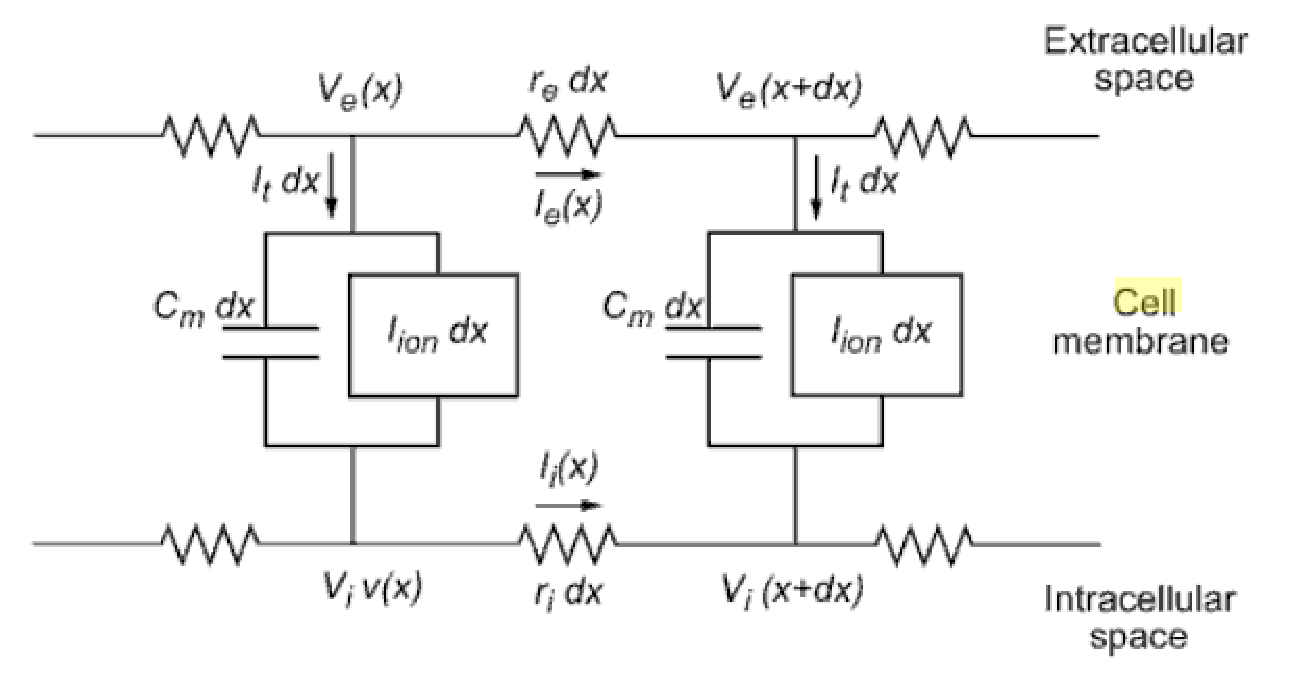
\includegraphics[height=4cm,
    angle=0]{./images/cable_circuit.eps}}
  \caption{Schematic diagram of the first discretized cable section of
    length $dx$}
\label{fig:cable_circuit}
\end{figure}
% 
% Consider the length is $l$, with cross-sectional area is $A_i$, and finite
% extracellular space with a cross-sectional area is $A_e$,  the resistivity
% $r_i, r_e$ are
% \begin{equation}
% r_i = \frac{R_i.l}{A_i} \;\;\;; \;\;\; r_e=\frac{R_e.l}{A_e}  
% \end{equation}
% \begin{enumerate}
% \item $r_i$: internal resistance per a unit length of cylinder (Ohm/cm)
% 
% The interior fluid with conductivity (electrical resistivity) $\rho_i$, axon
% radius to outside membrane $a$ and length of the cable $L$
% \begin{equation}
% R_i = \frac{\rho_i . L}{\pi a^2}
% \end{equation}
% $\rho_i = 0.5 \Omega.m$. \textcolor{red}{The internal resistance increase with
% decreasing radius $a$}
% \begin{equation}
% r_i = \frac{\rho_i }{\pi  a^2}
% \end{equation}
% 
% \item $r_e=0$: external resistance per a unit length of cylinder (Ohm/cm), if
% $A_e=\infty$
% \end{enumerate}
% In the absence of a connection between the extracellular and the intracellular
% spaces, the current $i_i$ and $i_e$ are constants, and the transmembrane
% potential $V_m$ (as well as electrical field E) are maintained.


The cable model is based on an infinitely long fibre with a uniform
cross-section. An electric circuit analogy of such fibre is given in Fig.
\ref{fig:cylinder}. The membrane potential, of course, is non-isopotential, and
is a function of length from the origin. The theory of flow of electricity in a
leaky cable dates back to the work of Lord Kelvin in 1855. However, its
application to neuronal behavior is mainly due to Hodgkin and Ruston
(1946)\citep{hodgkin1946ecc} with their ``theory of axonal
electrotonus''\footnote{electrotonus refers to the subthreshold (or
  linear) condition}
and later with a series of papers by Rall (1957, 1959, 1960,
1969)~\citep{segev1994fdf}.
% Thus, after the pioneering work of Wilfrid Rall (1950s and 1960s) that applied
% the theory of {\bf cable equation} to cell bioelectricity, the importance of
% spatial effects has been widely recognized.


% TODO: convert to the same conventions being used in the 2 previous sections





If the cable segment i-th has the cross section area $A_i$, then the
resistance per unit cross section area is
\begin{eqnarray}
  \label{eq:423}
  r_i = \frac{R_c}{A_i} \left( = \frac{R_i}{A_i} \right)
\end{eqnarray}
with $R_c$ (or $R_i$) is the {\bf cytoplasmic resistivity} or internal
resistivity (Ohm.mm).

\textcolor{red}{The change (decrease) in the intracellular current (cytoplasmic
current) is due to the leak currents through the membrane} $i_m$ (mA/cm) known
as the (positive outward) transmembrane current per unit length of the membrane 
\begin{eqnarray}
  \label{eq:424}
 i_m dx =  I_i(x) - I_i(x+dx) 
% I_m = I_tdx =  I_i(x) - I_i(x+dx)  = I_e(x+dx) - I_e(x)
\end{eqnarray}

% with $I_t$ is the total transmembrane current per unit length of
% membrane (mA/cm), $I_m$ is the .

In the limit  $dx\rightarrow 0$, 
\begin{eqnarray}
  \label{eq:426}
  i_m = - \frac{\partial I_i}{\partial x}
\end{eqnarray}
The applied current density is expressed as a current per unit length,
$i_p$ (negative inward) to have the same unit as $i_m$. % As $I_p$ enter
% the extracellular space and divided into the intracellular component
% $I_i$ and extracellular component $I_e$. 
The increase in extracellular current is due to the leak current
(positive outward) plus the (negative inward) stimulus current.
\begin{eqnarray}
  \label{eq:495}
  (i_m + i_p)dx = I_e(x+dx) - I_e(x)
\end{eqnarray}
then
\begin{eqnarray}
  \label{eq:496}
  i_m+i_p = \frac{\partial I_e}{\partial x}
\end{eqnarray}

The total axial current at each point along the fiber is composed of
the intracellular, extracellular: $I_T = I_i + I_e$ which is constant,
thus
\begin{eqnarray}
  \label{eq:498}
  \frac{\partial I_T}{\partial x} = (i_m+i_p)-i_m = i_p
\end{eqnarray}
% which means the total axial current is equal to the applied current
% $I_p=i_p\times dx$. 

{\bf Axial currents linked to transmembrane potentials}
With $V_m=V_i-V_e$, then using eq.~\eqref{eq:422}, we have
\begin{eqnarray}
  \label{eq:499}
  \frac{\partial V_m}{\partial x} &=& - r_iI_i + r_eI_e = -r_iI_i +
  r_e(I_T-I_i) \\
 &=&  -(r_i+r_e)I_i + r_eI_T
\end{eqnarray}
Thus
\begin{eqnarray}
  \label{eq:500}
  I_i = \frac{-1}{r_i+r_e}\left[\frac{\partial V_m}{\partial x} - r_eI_T\right]
\end{eqnarray}
then combine with eq.~\eqref{eq:426}, we have
\begin{eqnarray}
  \label{eq:501}
  i_m  = \frac{\partial}{\partial x}\left(\frac{1}{r_i+r_e}\left[\frac{\partial V_m}{\partial x} - r_eI_T\right]\right)
\end{eqnarray}
Under the condition of subthreshold, $r_i, r_e$ are both constant and
since $\frac{\partial I_T}{\partial x} = i_p$, we have the reduced form
\begin{eqnarray}
  \label{eq:429}
   i_m  &=& \frac{1}{r_i+r_e} \left[\frac{\partial}{\partial
     x}\left(\frac{\partial V_m}{\partial x}\right)
   - r_ei_p \right]\\ 
   &=&  \frac{1}{r_i+r_e} \left(\frac{\partial^2 V_m}{\partial x^2}
   - r_ei_p \right)\\ 
\end{eqnarray}

\textbullet If there is no stimulus current ($i_p=0$), we have
\begin{eqnarray}
  \label{eq:502}
    i_m  &=&  \frac{1}{r_i+r_e} \left(\frac{\partial^2 V_m}{\partial x^2}
    \right)
\end{eqnarray}


In addition, $i_m$, the total transmembrane current (positive outward)
per unit length, is also the sum of the capacitive and ionic current
\begin{eqnarray}
  \label{eq:425}
  i_m = p(\Cm\frac{\partial V_m}{\partial t} + I_{ion})
\end{eqnarray}
with $p$ is the perimeter of the cable (mm$^2$), and $\Cm$ is the
capacitance per unit area of membrane (C/mm$^2$) and $I_{ion}$ has
unit of current per unit area (mA/mm$^2$). $V_m=V_i-V_e$ is the
membrane potential, i.e. the difference between internal and external
voltage.

Combining eq.~\eqref{eq:502} and eq.~\eqref{eq:425}, we have the
complete form of the {\bf cable equation} is
\begin{eqnarray}
\label{eq:430}
  i_m = p(\Cm\frac{\partial V_m}{\partial t} + I_{ion}) =  \frac{1}{r_i+r_e} \left(\frac{\partial^2 V_m}{\partial x^2}\right)
%  \frac{\partial}{\partial x}\left(
    % \frac{1}{r_i+r_e}\frac{\partial V_m}{\partial x} \right)
\end{eqnarray}

\textbullet \textcolor{red}{If there is a current $i_p$ injected into the cell,
the total transmembrane current} is given
\begin{eqnarray}
  \label{eq:431}
  i_m = p(\Cm\frac{\partial V_m}{\partial t} + I_{ion} + I_p) =
  \frac{1}{r_i+r_e} \left(\frac{\partial^2 V_m}{\partial x^2} - r_ei_p\right) 
  % \frac{\partial}{\partial x}\left( 
  %   \frac{\partial V_m}{\partial x} -r_ei_p\right)
\end{eqnarray}
with $p$ is the perimeter of the cable (mm$^2$), and $\Cm$ is the
capacitance per unit area of membrane (C/mm$^2$) and $I_{ion}$ has
unit of current per unit area (mA/mm$^2$).


The transmembrane resistance per unit length is
\begin{eqnarray}
  \label{eq:455}
  r_m=\frac{R_m}{p}
\end{eqnarray}
with $p=2\pi a$ the area of the cross section, and $R_m$ is the
{\bf membrane resistivity}, i.e. resistance for a unit square area of
the membrane (Ohm.mm$^2$), then for any fixed membrane voltage $V_0$,
$R_m$ is determined by measuring the change in membrane current when
$V_m$ is perturbed slightly from $V_0$.
\begin{eqnarray}
  \label{eq:432}
  \frac{1}{R_m} = \frac{dI_{ion}}{dV_m}|_{V_m=V_0}
\end{eqnarray}

As $R_m$ depends on the chosen value $V_0$, it is typical to choose
$V_0$ as the resting potential to define $R_m$. However, for the
underthreshold condition, the membrane is an ohmic resistor, then we
don't need to define $V_0$, as
\begin{eqnarray}
  \label{eq:434}
  R_m = V_m/I_{ion}
\end{eqnarray}

Again, with underthreshold condition, $r_i, r_e$ are constant, then
combining with eq.~\eqref{eq:430}, a new form of the cable equation is
\begin{equation}
  \label{eq:433}
  \begin{split}
    R_m\Cm\frac{\partial V_m}{\partial t} + R_mI_{ion} &=
    \frac{R_m}{p(r_i+r_e)}  \frac{\partial^2V_m}{\partial x^2}\\
    \tau_m\frac{\partial V_m}{\partial t} + R_mI_{ion} &=
    \lambda_m^2  \frac{\partial^2V_m}{\partial x^2}\\
  \end{split}
\end{equation}
with $\lambda$ is the cylindrical cable's {\bf space constant} or
{\bf characteristic length}
\begin{eqnarray}
  \label{eq:447}
  \lambda = \sqrt{\frac{R_m}{p(r_i+r_e)}} =  \sqrt{\frac{r_m}{(r_i+r_e)}}
\end{eqnarray}
with the unit of distance; and
\begin{eqnarray}
  \label{eq:448}
  \tau_m=R_m\Cm
\end{eqnarray}
has unit of time and thus is called {\bf time constant}.

If we ignore the extracellular resistance ($r_e=0$), then using
eq.~\eqref{eq:423}, and $A_i=\pi a^2$, $p=2\pi a$ (with $a$ is the
radius of the cable), we have a simplified form of eq.~\eqref{eq:447}
\begin{eqnarray}
  \label{eq:449}
  \lambda_m =  \sqrt{\frac{R_m d}{4R_i}}
\end{eqnarray}
with $d=2a$ is the diameter of the
cable.
\textcolor{red}{Eq.~\eqref{eq:448} and eq.~\eqref{eq:449} are very
  widely used in computational physiology}.


Thus, eq.~\eqref{eq:433} is equivalent to the widely used form
\begin{eqnarray}
  \label{eq:558}
  \Cm\frac{\partial V_m}{\partial t} + I_{ion} =
  \frac{d}{4R_i}\frac{\partial V_m^2}{\partial x^2}
\end{eqnarray}


The ionic current $I_{ion}$ consist of leakage, synaptic, and
intrinsic membrane currents (Na, K, Ca). The synaptic current is
\begin{eqnarray}
  \label{eq:559}
  I_{synaptic} = g_{synaptic}(t).(V-V_{r,synaptic})
\end{eqnarray}
with $V_{r,synaptic}$ is the reversal constant potential
characteristic to the type of synapse, and conductance is time
dependent only. However,
\textcolor{red}{Many synapse conductances, e.g. GABA-activated
  Cl-channel, NMDA-activated channels have a more complex dependence
  voltage $V_m$}.
The leakage or intrinsic membrane current have the similar formula as
above, yet the conductance can be both time and voltage-dependent
(read Hodgkin-Huxley model).
\begin{eqnarray}
  \label{eq:560}
  I_{active} = g_{active}(t, V).(V-V_{r,active})
\end{eqnarray}



In the subthreshold condition, and no synaptic or active (ionic)
currents other than leakage current,
i.e. $f=-I_{leak}.R_m=V_m$. Typical values for the parameters are
shown in Fig.~\ref{fig:param_cell}.


Eq.~\eqref{eq:436} can be transformed into the classical 1D heat
equation
\begin{eqnarray}
  \label{eq:562}
  V_m(X,T) = U(X,T) e^{-T}
\end{eqnarray}





\section{How to incorporate discrete elements into continuum models}



\section{Whole-heart modelling}
\label{sec:whole-heart-modelling}

The number of cells in a cardiac cells is much larger than the number being used
in very large models like $10^5$ cells \citep{muller-borrer1994}. To avoid
computational demand, simple single-cell models are of widely used.
The first simple two-state model is the Fitzugh-Nagumo model (1961) to describe
excitability phenomena and AP generation (Sect.\ref{sec:fitzh-nagumo-model}).
Newer simple models to improve the qualitative behaviors, like shape of AP,
pacemaker activity, have been developed, e.g. van Capelle-Durrer
(Sect.\ref{sec:vanCapelle-Durrer}), Aliev-Panfilov
(Sect.\ref{sec:aliev-panfilov}), Mitchell-Schaeffer
(Sect.\ref{sec:mitchell-schaeffer}), Djabella-Landau-Sorine
(Sect.\ref{sec:djabella2007}).
 
The network models consider single cells discretely
(Sect.\ref{sec:tissue-modelling}). However, it remains infeasible to solve for
cardiac activity at whole-heart level using this approach. Also, this type of
approach is not suitable for investigation of mechanical behavior of cardiac
tissue unless the dynamics of intracellular and extracellular components need to
couple with mechanical components of the cells.

Current approach at whole-heart modelling is based on continuum modelling,
allowing detailed cell models to be incorporated and propagated throughout the
whole organs. This make it easier to incorporate the electrical activity to the
mechanical activity of the tissue. However, it's still available to incorporate
the discrete elements into continuum models.
Early works include \citep{leGrice1992}.   


\section{PDE in physical models}

Second-order PDEs commonly arise in physical models.
\begin{enumerate}
  \item Elliptic PDE, e.g. Poisson equation $\nabla^2 u + g = 0$, when $g=0$, it
  becomes Laplace equation $\nabla^2u=0$
  
  E.g.: In electric potential, the electric field E is related to the charge
  density: $\nabla E = \frac{\rho}{\varepsilon_0}$ (with $\rho$=charge density,
  $\varepsilon_0$=permitivity, while E is related to the electric potential by
  $E=-\nabla V$, so $\nabla^ V=-\frac{\rho}{\varepsilon_0}$. In the charge-free
  region of space, then $\nabla^2 V = 0$.
  
  \item Parabolic PDE, e.g. heat equation $u_t = \nabla^2 u + g$
  \item Hyperbolic PDE, e.g. wave equation $u_{tt}=\nabla^2u$
\end{enumerate}

A PDE can be in either strong form or weak form. A strong form of the PDE
requires that the solution have a second derivative. A weak form only requires
first derivative to be existed. To convert from strong form to weak form, we can
\begin{enumerate}
  \item Multiply ODE by a virtual function $u^v(x)$, satisfying $u^v(0)=0$
  \item Shift derivatives: 
  \item Integrate
  \item Apply boudary conditions
  \item Arrive at weak statement
\end{enumerate}
The reason of using weak form is that it's difficult to integrate the strong
form equation to obtain the exact solution, e.g.
\begin{equation}
\nabla^2 u = \frac{-1}{1+x^2}; u(0)=0, u(1)=0
\end{equation}
If we try an approximate solution $u(x)=Ax+Bx^2$ with A,B are constants
satisfying the boundary condition. When we substitute to the strong form, we get
\begin{equation}
-B=\frac{-1}{1+x^2} \;\;\;; A+2B=0
\end{equation}
which makes B not a constant.

If we substitute into the weak form, we get $u(x)\approx -0.75x+0.4x^2$.


For solving nonlinear PDE, e.g. $-\nabla y +f(y)=0$, there are two common
approaches:
\begin{enumerate}
  \item Fixed point iteration: choose an initial value $y^0$, then
  iteratively solve until the system converge, i.e. $|y^{k+1}-y^k|\le
  \varepsilon$
  \begin{equation}
  -\nabla y^{k+1}+f(y^k)=0
  \end{equation}
  Here, $y$ is replaced by $y^{(k+1)}$ in all linear terms, and by $y^{k}$ in
  all nonlinear terms. 
  
  \item Newton method: choose an initial value $y^0$
  \begin{equation}
  -\nabla \delta y + f'(y^{k})\delta y = - \left( \nabla y^{(k)} + f(y^{(k)})
  \right)
  \end{equation}
  and set $y^{(k+1)}=y^{(k)}+\delta y$. So, how to compute $\delta y$. There are
  difference choices; the easiest and least error-prone is to apply
  finite-difference discretization in time by the so-called $\theta$ method and
  solve the discretized problem.
  \begin{equation}
  \frac{y^{n+1}-y^{n}}{\Delta t} + (1-\theta) f^{(n+1)} + \theta f^{n} = 0 
  \end{equation}
  and
  \begin{equation}
  h^{(n+1)} + (1-\theta) \Delta t f^{(n+1)} = h^n - \theta \Delta t f^{(n)}
  \end{equation}
  Now, to apply Newton's method, we need to linearize $h^{(n+1)}$ by assuming
  $h^{(n+1)}= h^* + c$, with $h^*$ is a guess of the solution, and $c$ is the
  correction. Then, using Taylor's expansion, the nonlinear part is approximated
  by
  \begin{equation}	
  f^{(n+1)}=f(h^{(n+1)})\approx f(h^*+c) = f(h^*) + J_f(h^*).c = f^* + J^*_f.c
  \end{equation}
  with $J_f$ is the Jacobian matrix for function $f$, and $J^*_f=J_f(h^*)$.
  Finally, a system of linear equations is
  \begin{equation}
  \left( I + (1-\theta) \Delta t J^*_f  \right) c = -h^* - (1-\theta) \Delta f^*
  + h^n - \theta \Delta t f^n
  \end{equation}
  After each time step, we need to keep correcting the guess solution until the
  correction term $c$ is small enough.
  
  
\end{enumerate}
The choosing of which method to use depends on the non-linear term $f$. However,
fixed-point is typically not a method of choice for practical applications. So,
standard method for solving nonlinear PDE is Newton method which involves 2
steps: (1) numerical discretization to get a set of nonlinear algebraic
equations, (2) application of the Newton iterative linearization techniques or
its variants to solve the nonlinear algebraic systems. Other techniques
\begin{enumerate}
  \item Direct Linearization Method (DLM): a nonlinear term is considered as a
  new independent systematic variable and transfer a nonlinear PDE into a linear
  PDE with more than one independent variable \citep{chen2001}.
  \item 
\end{enumerate}

\subsection{FEM and FDM}

FEM (Finite Element Method) and FDM (Finite Difference Method) are suitable only
for linear PDE. But in cardiac electrophysiological modelling, we have nonlinear
PDE. So we need to linearize it first.

FEM can handle better boundary problems where odd geometries exist or it's
easier to make more finer subdivisions of the space in regions where we need
more accuracy. However, tuning the code in FEM is not easy, compared to FDM.

\subsection{Monodomain and Bidomain for cardiac eletrophysiology}

The monodomain equation is essentially a heat equation coupled to an ODEs (with
variable in the ODEs are ionic current parameters)
\begin{equation}
\begin{split}
\chi \left( \Csc \frac{\partial V_m}{\partial t} + I_\ion (\mathbf{u}, V_m)
\right)  - \nabla \cdot (\sigma \nabla V_m) = 0 \\
\frac{\mathbf{u}}{dt} = \mathbf{f(u}, V)
\end{split}
\end{equation}
Here the boundary is zero-Neumann boundary conditions.

The electrical properties of the myocardium are generally described by the bidomain
equations, a set of coupled parabolic and elliptic partial differential
equations (PDEs) that represents the tissue as two separate, distinct continua -
one intracellular and the other extracellular.   The intracellular and the
extracellular media are connected via the cell membrane, and thus the two PDEs
are coupled at each point in space through a set of complex, non-linear ordinary
differential equations (ODEs), which describe the ionic transport across the
cell membrane.

The bidomain equation is written in the form of parabolic PDE coupled to
elliptic PDE coupled to ODEs (i.e. 3 sets of equations)
\begin{equation}
\begin{split}
\chi \left( \Csc \frac{\partial V_m}{\partial t} +  \right) - \nabla \cdot
\left( \sigma_i \nabla (V_m + \phi_e) \right) = 0 \\
\nabla \cdot \left( \sigma_i \nabla V_m + (\sigma_i + \sigma_e ) \nabla \phi_e
\right) = 0 \\
\frac{d\mathbf{u}}{dt} = \mathbf{f(u,}V)
\end{split}
\end{equation}
Here the boundary is zero-Neumann boundary conditions.
												


\subsection{Chaste Implementation}

They developed abstract classes with abstract methods from which you can derive
the proper for your problem and implement thems
\begin{verbatim}
AbstractLinearEllipticPde
   Abs. method: GetDiffusionTensor(x)
   Abs. method: GetForceTerm(x)
   
\end{verbatim}

Then, we develop our class for the problem 
\begin{verbatim}
MyEllipticPde: inherets from AbstractLinearEllipticPde
   Implement method: GetDiffusionTensor(x)
   Implement method: GetForceTerm(x)
\end{verbatim}
In the case of $\nabla^2u = 0$, then \verb!GetDiffusionTensor(x)! should return
an identity matrix, and \verb!GetForceTerm(x)! should return zero.
 
\section{FD methods}

A regular grid of evenly spaced solution points are distributed across the
solution domain. Each partial derivative in the activation equations is then
approximated by a {\it finite-difference}, e.g. a truncated form of Taylor's
series expansion of the dependent variable in terms of values at neighbouring
points.

Examples of bidomain FD implementations restricted to regular and uniform
meshes: \citep{Latimer1998, Quan1998, Skouibine1999}. 


\citep{Huiskamp1998, Weixue1996} used a small enough grid-point with a cubic box
enclosing the geometry. An individual value (with total 255 values representing
255 different directions) was assigned to each grid-point. Nevertheless, at some
boundary points, the jagged on angled or curve-boundary may affect the
calculations.

\citep{Cherry2000, Cherry2000b} used a governing capacity functions that has the
value 1 if the gridpoint lies within the solution domain and 0 if outside the
solution domain. If the domain boundary crosses the cell then the capacity
function get a value in the range (0,1) that represents the portion of the cell
within the solution domain. However, the method doesn't work well with
deformation where the problem domain can become irregular.

\section{Finite-element methods}
\label{sec:finite-element-method}



\section{Finite-difference methods}
\label{sec:finite-difference-method}

FE method discretizes the solution domain into elements and interpolates nodal
values over each element using a basis function, e.g. a cubic Hermite function.
The method works well with irregular domain. 

\section{Finite-volume method}
\label{sec:finite-volume-methods}

Finite-volume methods (FVM) - sometimes also called box methods - are
mainly employed for the numerical solution of problems in fluid mechanics, first
introduced in 1970s by McDonald, MacCormack, and
Paullay.
\begin{itemize}
  \item  \citep{Harrild1997} used the method for 2D.
  
  \item  \citep{Harrild2000fm} used the method for 3D.
\end{itemize} 

An important property of finite-volume methods is that the balance principles,
which are the basis for the mathematical modelling of continuum mechanical
problems, per definition, also are fulfilled for the discrete equations
(conservativity)


\section{FE-based FD method}
\label{sec:FE-based_FD}

Finite-Element (FE) based Finite-Difference (FD) Method ia a very general
framework to solve the bidomain equations (a system of PDEs) using FE to model
complex geometries and then using FD to solve it quickly. To provide local
behavior with a small space constant, the activation equations are solved on a
high resolution \textcolor{blue}{nonuniform FD grid} which is defined from and
embedded in the material space of the FEs. So, the PDEs can be solved using the
FD scheme, but the solution mesh is defined by the geometry of the problem
domain. So, any change to the geomtry due to deformation are tracked and then
applied to the host FE mesh as the material points remain invariants.



The FD mesh can be generated over a curve domain using FE interpolation by a
bais function, e.g. {\it cubic Hermite} (Sect.\ref{sec:Hermite_element}). 



\subsection{Hermite element}
\label{sec:Hermite_element}

High-order cubic Hermite finite element interpolation schemes have been used
widely in ventricular finite element modelling to capture smooth geometries with
few finite elements.

\section{Rudy-Quan (1987)}
\label{sec:rudy-quan-1987}

The anatomy structure of the myocardium as an assembly of discrete cells
separated by a periodic intercalated disk structure was established in 1954.
This discontinuous was not considered importance and thus modelling so far based
on the continuous model utilized successfully for nerves, e.g. one-dimensional
continuous cable theory \citep{jack1975}. This inhibited the investigation of
propagation phenomena like {\it slow conduction}, decremental conduction, {\it
conduction block}, and changes in APD and refractory periods. All of them are
considered important in causing reentrant arrhythmias. 

Using continuous cable theory is not adequate to explain phenomena in the heart.
Such as the maximum rate of change of the temporal AP $\dot{V}_\max$ displayed a
biphasic behavior as a function of increasing intercalated disk resistance. 
\citep{joyner1982} studied the discontinuity by discretizing the continuous
cable into elements of length $\Delta x$ (equal to the cell length). However,
they lumped together the myoplasmic resistance and the intercalated disk
resistance as $R_i$.

\citep{rudy1987} proposed a 1D discontinuous model to study the effect of
periodic intercalated disk structure on propagation in cardiac muscle. Each
element is of the same dimension of a cell (100$\mum$ in length and $16\mum$ in
diameter), Fig.\ref{fig:cablemodel_Rudy1987}. Here, the myoplasmic resistance
and the intercalated disk resistance for each cell are two different variables.
In ischemia and infarction, disk resistance is abnormally high. Also, the
effect of increase leakage to the extracellular space can be simulated as what
occurs in areas of damaged in myocardium.

It's assumed that the interaction between cells is passive and the junctional
axial resistance is constant over a wide range of voltages. Also, capacitive
shuting is ignored. The model for each cell is based on \citep{beeler1977rap}
(Sect.\ref{sec:beeler-reuter-model}) as three membrane patches; and the core
conduction model \citep{hodgkin1946ecc}. Consider the boundary condition: for a
symmetrical finite length fiber, the boundary condition at the stimulating
electrode (x=0) is $V_{-j}=V_{j}$ (symmetry w.r.t x=0), while at the other end,
$\partial V_m/\partial x=0$ (a sealed end).

\begin{figure}[hbt]
  \centerline{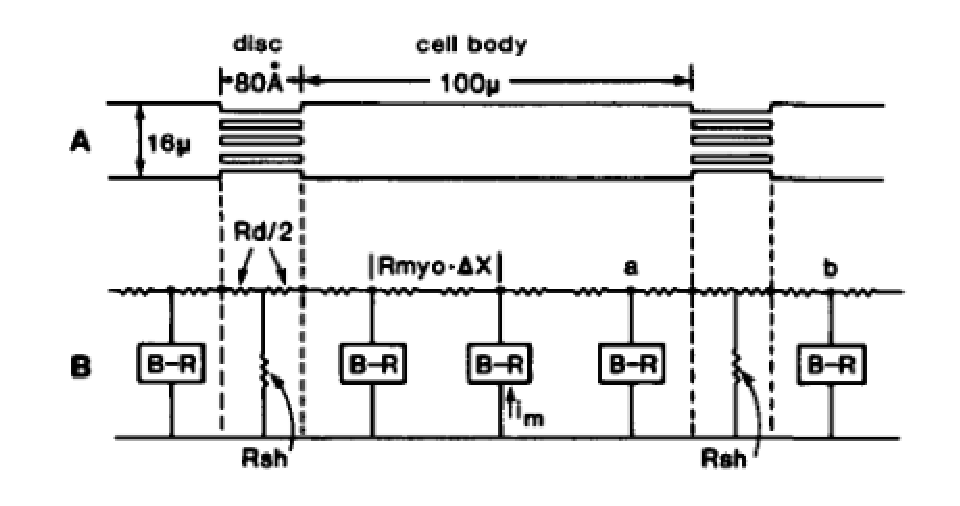
\includegraphics[height=5cm]{./images/Cablemodel_Rudy1987.eps}}
\caption{(A) A discrete cable model of cylindrical cardiac cells
\citep{rudy1987}; (B) Core conductor network with 3 Beeler-Reuter membrane
paches per cell; a T-network representing the intercalated disk between cells
$R_d$, myoplasmic resistivity $R_\myo$, and leakage resistance to extracellular
space $R_\text{sh}$}
\label{fig:cablemodel_Rudy1987}
\end{figure}




\subsection{Mathematical model}

A 1D fiber of 40-100 cells. Neighboring cells are coupled through an
intercalated disk modeled as a T-resistance network with 2 axial resistance
representing the intercytoplasmic channels [connexons], and a radial leakage
resistance to the extracellular space, Fig.\ref{fig:cablemodel_Rudy1987}. 

The equation for propagating AP $V_m(x,t)$ at every cell is given by
\begin{equation}
\frac{r}{2}\frac{1}{R_i+R_e}\frac{\partial^2 V_m(x,t)}{\partial x^2} = \Csc
\frac{\partial V_m(x,t)}{\partial t} + I_\ion + I_\app
\end{equation}
% NOTE: If $R_i,R_e$ are cell-specific, then we need to put $1/(R_i+R_e)$ into the
% second-order derivative
with $r$ is the radius of the fiber; $R_i, R_e$ are internal and external
resistance, respectively. The term $I_\ion$ are 4 individual ionic
currents. $I_\app$ is the stimulus current.

The transmembrane potential $V_m$ is calculated based on the method described in
the next section. The extracellular potential field of a uniform cylindrical
fiber in a conducting medium of conductivity $\sigma_e$ can be computed from
$V_m$ using the following integral formula \citep{plonsey1977}
\begin{equation}
\label{eq:extracellular_potential-field}
\Phi = -\frac{\sigma_i}{4\pi \sigma_e} \int dA \int \frac{\partial
V_m}{\partial X} \vec{a}_x .\nabla\left(\frac{1}{r}\right) dx
\end{equation}
with $\sigma_i$ is intracellular conductivity, $\vec{a}_x$ is the unit vector
in the direction of fiber axis, $r$ is the distance from the source point to the
field point. IMPORTANT: big $X$ represents the axial direction distance (cross
section; while small $x$ represent longitudinal direction distance). Here, the
source is very large at the disk. The formula can be discretized into the
contribution from the cells and from the junction with a different cross
section: $A_m$ (myoplasm), $A_j$ (junction). So, for a single  cell, the
extracellular potential field is 
\begin{equation}
\Phi = -\frac{\sigma_i}{4\pi \sigma_e} \left[ \int dA_m \int_m \frac{\partial
V_m}{\partial X} \vec{a}_x .\nabla\left(\frac{1}{r}\right) dx
+ \int dA_j \int_j \frac{\partial
V_m}{\partial X} \vec{a}_x .\nabla\left(\frac{1}{r}\right) dx 
\right]
\end{equation}
Typically, the  cross-sectional area $A_j$ is only 0.03\% of the cell body
cross-sectional area $A_m$. \textcolor{red}{The total extracellular potential
is the summation of all $\Phi_i$ in all cells}.
NOTE: $-\partial V_m/\partial X$ and $i_m$ are related by the cable equation,
with $i_m$ is the transmembrane current per unit length. So with $r_i$ is the
intracellular axial resistance per unit length of the fiber, we can use
\begin{equation}
\Phi = \frac{\sigma_i}{4\pi \sigma_e}\int dA \int \frac{r_i.i_m}{r}dx
\end{equation}

\subsection{Numerical method}

The discretization of the second partial derivative is based on the second order
central difference formula
\begin{equation}
\frac{\partial^2 V_m(x,t)}{\partial x^2} = \frac{V_{j+1}^k - 2 V_j^k +
V_{j-1}^k}{(\Delta x)^2}
\end{equation}

However, this formula is not valid at junctional points, such as (a) and (b) in
Fig.\ref{fig:cablemodel_Rudy1987}(B). To take into account the assymetry in the
resistance
\begin{enumerate}
  \item For point (a): we use
  \begin{equation}
  \frac{2V_{j+1}^k - 3 V_{j}^k + V_{j-1}^k}{(\Delta x)^2}
  \end{equation}
  \item For point (b): we use
  \begin{equation}
  \frac{2V_{j-1}^k - 3 V_{j}^k + V_{j+1}^k}{(\Delta x)^2}
  \end{equation}
\end{enumerate}


\section{Leon-Roberge (1991)}

\citep{leon1991} 

\citep{leon1994} 

\section{Nesterenko-Antzelevitch (1992) U-wave}

\citep{nesterenko1992}  analyzed the cell-to-cell coupling, transmural
dispersion of APD, and electrocardiographic U wave in 1D cable. U-wave is a
small (0.5mm) deflection immediately following the T-wave, usually in the same
direction as the T-wave (which is best seen in leads V2 and V3). The source of
the U-wave is unknown, while there are 3 common theories:
\begin{enumerate}
  \item delayed repolarization of Purkinje fibers
  \item prolonged repolarization of the mid-myocardial M-cells
  \item after-potential (EAD or DAD) resulting from mechanical forces in the
  ventricular wall.
\end{enumerate}
IMPORTANT: U-wave is inversely proportional to heart rate, i.e. U-wave grows
bigger with slower heart rate (and generally become visible when heart rate
falls below 65bpm). Voltage fo U-wave is typically $<25\%$ of T-wave voltage. On
ECG, maximum normal amplitude of the U-wave is 1-2mm. Under pathophysiological
conditions, U-wave can be prominent ($>1-2$mm or $>25\%$ of the height of the
T-wave: the most common cause is {\it bradycardia}, with abnormally prominent
is seen in severe hypokalaemia) and inverted (highly specific for the presence
of heart disease). Drugs can also cause prominent U-wave, e.g. digoxin, class Ia
antiarrhythmias (quinidine, procainamide), class III antiarrhythmias (sotalol,
amiodarone). Many conditions that cause prominent  U-wave also cause long-QT
syndrome. 

Single cell model is based on LR-1 model (Sect.\ref{sec:luo-rudy-phase-1}). The
authors assumed that the actual surface ECG arises mainly from LV and is the
result of a planar wavefronts conducting across the heart-wall from outside to
inside. Thus, a 1D cable is assumed enough to reasonably approximate ECG
characteristics.

To reproduce the normal transmural APD gradient, the maximum conductance
$\bar{g}_\k$ is gradually increased. A cell is assumed 100$\mum$ in length with
internal resistivity of 200 Ohm.cm are oriented along the longitudinal cable
axis, connected through gap junctions (2 Ohm.cm$^2$) at selected points along
the fiber. A 2cm linear cable comprised of 200 myocardial cells coupled through
gap-junctions. To emulate M-cell region (cells 100-160), $\bar{g}_\k$ of cells
in this region is statically uniformly reduced.

However, under the condition of intrinsic heterogeneity of APD (from 300ms to
550ms) and homogeneous cellular coupling, no U wave was observed in the
simulated ECG, no matter how great APD prolongation in M-region
\citep{nesterenko1992}. M-cells are thought to contribute 30-40\% of the ventricular wall, and
thus can contribute importantly to the body surface ECG. Thus, the authors
hypothesized that M-region is surrounded by high resistance barriers (increased
gap-junctional resistance) that cause a sharp transition in APD from Epicardium
to M-cells. 

The shape and amplitude of the simulated U-wave is examined as a function of (1)
resistance of M-region border, (2) the extent of prolongation of AP in the
M-region (up to 500ms), and (3) the physical size of M-region.

\subsection{Mathematical model}

The electrical activity propagated from one cell to another on a 1D cable is
given by the Hodgkin-Huxley equation (\ref{eq:cable_HH}), yet in a generalized
form with heterogeneous resistivity
\begin{equation}
I_\ion + \Csc \frac{\partial V_m}{\partial t} =
\frac{r}{2}.\frac{\partial}{\partial x}\left( \frac{1}{R(x)}.\frac{\partial
V_m}{\partial x} \right)
\end{equation}
with $r=0.0008$(cm) is the fiber radius, $r_i(x)$ is the local longitudinal
resistivity, $V_m$ is transmembrane potential, $\Csc=1\muF/$cm$^2$ is the
specific membrane capacitance.

Extracellular potential field was calculated based on \citep{rudy1987}
(Sect.\ref{sec:rudy-quan-1987}), eq.\ref{eq:extracellular_potential-field}.
However, to further simplify it, it's assumed that the observations are made at
a distant field point, i.e. $a_x.\nabla(1/r)$ can be considered as constant.
Also, inspite of the much larger spatial voltage gradient across the
gap-junction, the much smaller volume $A_j$ vs. $A_m$ make the contribution of
$A_j$ to the ECG is negligible. So, it's assumed that only voltage gradient
along the cell bodies actually contribute to ECG.

So, the voltage difference across the cell body $dV_c$ is also the transmembrane
potential $dV_m$
\begin{equation}
dV_c = \frac{R_m}{R_m+R_j} .dV
\end{equation}
with $R_m, R_j$ is myoplasmic resistance and junctional resistance,
respectively; $dV$ is the voltage difference between neighboring cells. 

\subsection{Simulation method}

$I_\app$ is given at cell 1 (endocardial side of the fibder). To simulate a
positive T-wave in the ECG, a constant gradient of the maximal delayed rectifier
conductance $G_x$ (in Luo-Rudy-1 model) was introduced, i.e. $G_x$ (cell-1) is
0.282 (giving APD=367ms), $G_x$ (cell-200) is 0.45 (giving APD=297ms).

Prolongation of the APD between cell 1 and cell 160 (M-region) was produced by a
uniform decrease of $G_x$.

\subsection{Numerical method}

Finite difference equation was solved using Crank-Nicolson method
(Sect.\ref{sec:Crank-Nicolson-method}) with $dt=10\mus$. The spatial resolution
was either 100$\mum$ or 20$\mum$, depending on the type of simulation. Spatial
resolution of 20$\mum$ was used to test the contribution of different region to
the ECG.

\subsection{Data analysis}

The result suggested the U-wave can be generated at least in part by the delayed
repolarization of M-cells found in the deep sub-epicardial to mid-myocardial
layers of the ventricular wall. 

When the resisistive barriers was imposed to partially insulate the M-region
from the remainder of the ventricular myocardium, the volume occupied by M-cells
was shown to be large enough to produce relatively large and distinct U-waves.

The hypothesis of Purkinjie fibers

\section{Karma (1993) - spiral wave}
\label{sec:karma1993}

\citep{Karma1993} 

\section{Muller-Borrer et al. (1994)}

\citep{muller-borrer1994}

\section{Trayanova (1996)}

\citep{trayanova1996}  

\section{Beaumont et al. (1998) - 2D spiral wave with stationary core}
\label{sec:beaumont1998}

\citep{beaumont1998}

\section{Chudin et al. (1998) - 2D wave propagation in VF}
\label{sec:chudin1998}

VF (ventricular fibrillation), the main cause of SCD (sudden cardiac death),
represents a severe distortion in wave propagation in the heart. The mechanism
was unknown as it can happen in a healthy heart or one with ischemia, i.e. 
the result of a damaged region of the cells.



\citep{chudin1998} developed a 2D tissue model of cardiac tissue, using
Luo-Rudy-2 (Sect.\ref{sec:luo-rudy-phase-2}) as the single cell model.

\section{Chudin et al. (1999) - VF in rabbits}
\label{sec:chudin-et-al}

During normal heart beats, myocardial cells undergo periodic
depolarizations of membrane potential, called AP. AP trigger the
influx of calcium via LCC, as well as calcium release from SR. The
shape of this AP waveform is determined by the ionic current across
the plasma membrane. Some of these fluxes, e.g. via LCC or NCX, are
controlled by the intracellular calcium concentration. Thus, calcium
system is driven by AP waveform that is itself dependent on the
dynamics of calcium system.

\textcolor{red}{The coupling between $V_m$ and intracellular calcium
  concentration is of particular important}.
This is known as
{\bf bidirectional coupling}. \citep{chudin1999icd} aimed to shed a light on
the mechanism by stimulating a rabbit ventricular myocyte using a clamped AP
waveform by using LR-2 model for each cell in the tissue of size . 

\citep{chudin1999icd} shown that 
\textcolor{red}{at high stimulation rates, the whole cell calcium
  transients exhibited {\bf alternans} even when the clamped voltage was
  periodic}. This suggested that the dynamically unstable in the calcium cycling is
independent of the dynamics of the membrane potential. Abnormalities in
calcium signaling could influence the membrane potential, and thus promote
arrhythmias.

They studied the mechanism for the transition from
ventricular fibrillation (VF) to VT using the hypothesis that high intracellular
calcium may trigger VF independently, i.e. affect the stability of the
spiral wave reentry.
\begin{enumerate}
\item measure $[\Ca]_i$ transient during high pacing comparable to VT

\item use the data above, and modify LR phase 2 model based
  on~\citep{luo1994dmc_a, zeng1995}: (1) reformulate relaxation of
  $\Ca_i$ and incorporate mechanism of $\Ca$ release from SR

\item simulate wave propagation in 2D uniform isotropic cardiac tissue
  to examine the stability of spiral wave reentry.
\end{enumerate}

\begin{figure}[hbt]
  \centerline{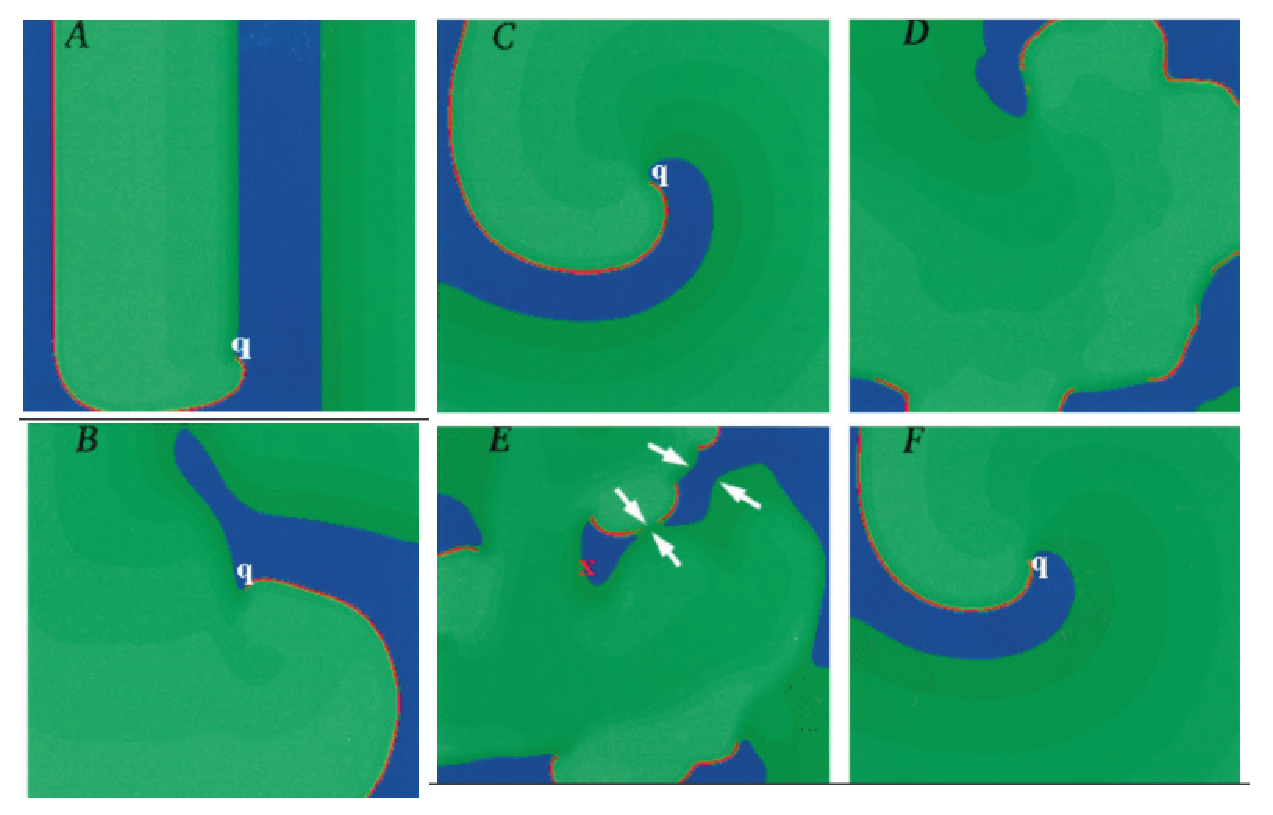
\includegraphics[height=5cm]{./images/Chudin_spiralwave.eps}}
\caption{Spiral waves}
\label{fig:Chudin_spiral}
\end{figure}



\subsection{Pacing protocol}
\label{sec:pacing-protocol}

Cells were paced sequentially for $\sim 16$ sec, following the cycle
length (in msec): 1000, 500, 400, 300, 180. 

The current clamp is twice the diastolic threshold in 2ms current
pulse. 

\subsection{Numerical analysis}
\label{sec:numerical-analysis-1}

The model was written in C++ and ported to massively parallel super-
computers: CRAY-T3E and HP-Exemplar. Typically, on 64 processors it
would require $\sim$20 min on CRAY-T3E and 40 min on HP-EXEMPLAR to
simulate 1sec of model time. 


Briefly, we used an operator splitting algorithm with a time step
varying between 0.005 and 0.1 ms and a fixed space step equal to 0.25
mm. Decreasing space step to 0.125 mm and minimal time step to 0.0005
ms did not significantly affect simulation results. The simulated
tissue was 64$\times$64 mm$^2$, larger than the critical size required to
support stationary and nonstationary wave circulation.

\subsection{Data analysis}
\label{sec:data-analysis-3}

APs were initiated with 30$\muA$/$\muF$ of $I_\stim$ during 1.3ms


\section{Viswanathan et al. (1999) - 190 cells forming 3 regions}
\label{sec:viswanathan-et-al}

With the justification that $I_\Kr$ and $I_\Ks$ play dominant roles in
repolarization of AP, ~\citep{viswanathan1999} examined how the change
in densities of these channels altered by diseases (e.g. long QT
syndromes like LQT1, LQT5, and LQT2) or by class III agents that
preferentially blocks one of these channels. 

This model is largely based on LR-2 model,
Fig.~\ref{fig:Viswanathan_model} (Sect.~\ref{sec:luo-rudy-phase-2}). 
The theoretical fiber is composed of 190 ventricular cells, each of
LRd formulation. In this fiber, cell 1-80 is endocardial region cells,
cells 81-110 is myocardial region cells, cells 111-190 is epicardial
region cells. In essence, we have 3 cells types: CT1, CT2, and CT3. 

\begin{figure}[hbt]
  \centerline{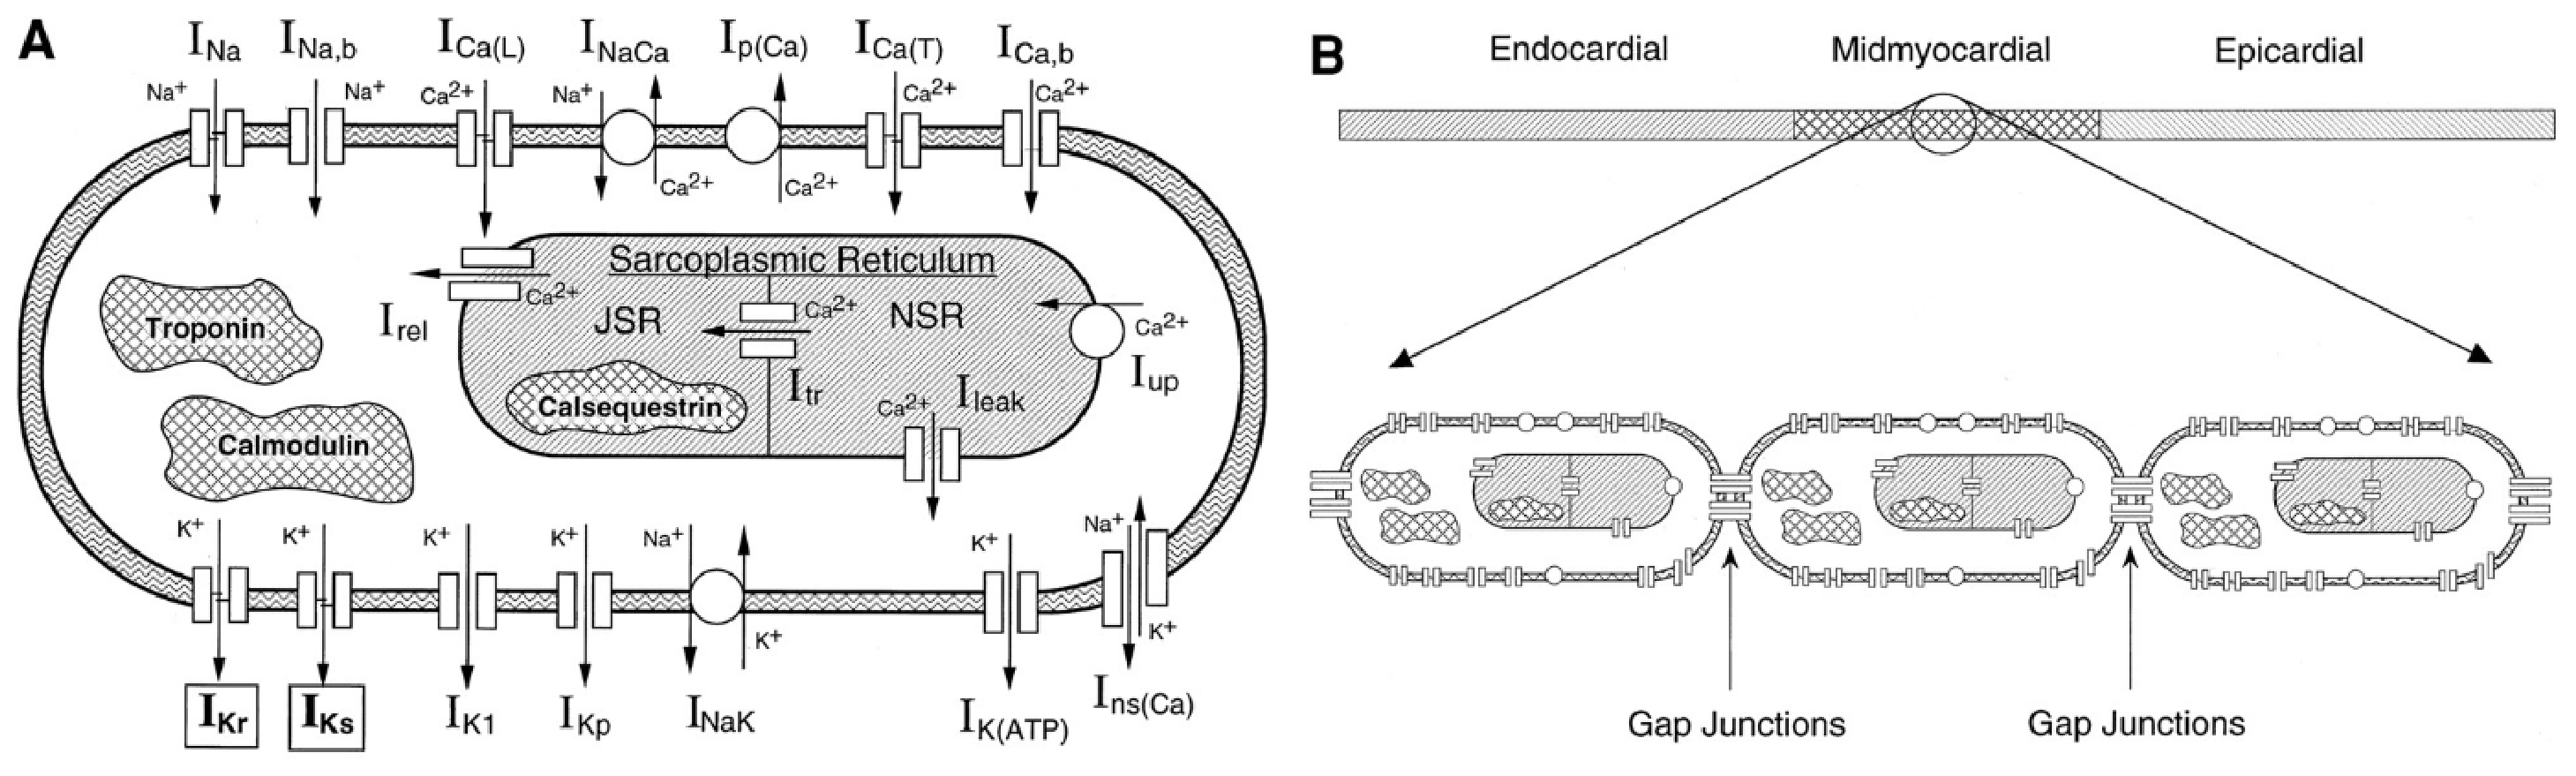
\includegraphics[height=4cm,
    angle=0]{./images/Viswanathan_model.eps}}
\caption{Schematic diagram of LRd model}
\label{fig:Viswanathan_model}
\end{figure}

The gap junction between cells is homogeneous throughout the fiber,
with 2.5$\mu$S (normal coupling) and 0.025$\mu$S (weak coupling). 

\subsection{Simulation protocol}
\label{sec:simulation-protocol}


Adaptation curves (the steady-state dependence of APD on rate) were
obtained by pacing the cell at a constant cycle length (CL) for 5
minutes to achieve steady state, followed by a step increase to the
next CL. APDs were obtained for CL of 300, 500, 800, 1000, 1500, 2000,
and 5000 ms. APD was measured between the time of stimulus onset and
90\% repolarization (APD90). All computations were performed at a
simulated temperature of 37$^\circ$C.

The fiber is paced (stimulated) from cell 1. 


They adjusted 
\begin{itemize}
\item Ks is decreased by 40\% and 80\% in CT2 and CT3 cells,
  respectively. 

\item IKr is similarly decreased in CT4 and CT5

\item ...

\end{itemize}

\section{Faber-Rudy model (2000) - role of $[\Na]_i$}
\label{sec:faber-rudy-model}


~\citep{faber2000} investigates the effect of elevated of $[\Na]_i$ on
AP and $[\Ca]_i$ using LR2 model (Sect.~\ref{sec:luo-rudy-phase-2}), a
long with some updates from~\citep{zeng1995}
(Sect.~\ref{sec:zeng-et-al}) and~\citep{viswanathan1999}
(Sect.~\ref{sec:viswanathan-et-al}).

In cardiac cells, Na/K and Na/Ca are the two important ion-regulating
transporters in maintaining the ionic balance across a cardiac
myocyte membrane. Rapid pacing and fast rates increase the $\Na$ and
$\Ca$ influx to an extent that these transporters can not restore the
ionic balance to a normal level.  This paper studied how the elevation
of $[\Na]_i$ and $[\Ca]_i$ relate to tachycardia and fibrillation. 

Special attention is given to $I_\NaCa$ and $I_\NaK$, as well as
$I_{\k(\na)}$ to AP shortening during $\Na$ overload. 

\subsection{Hypothesis analysis}
\label{sec:hypothesis-analysis-16}

New components: sodium-activate K channel $I_{\k(\na)}$, and
ATP-sensitive K channel $I_{\k(\ATP)}$~\citep{sanguinetti1990naa}.
\begin{figure}[hbt]
  \centerline{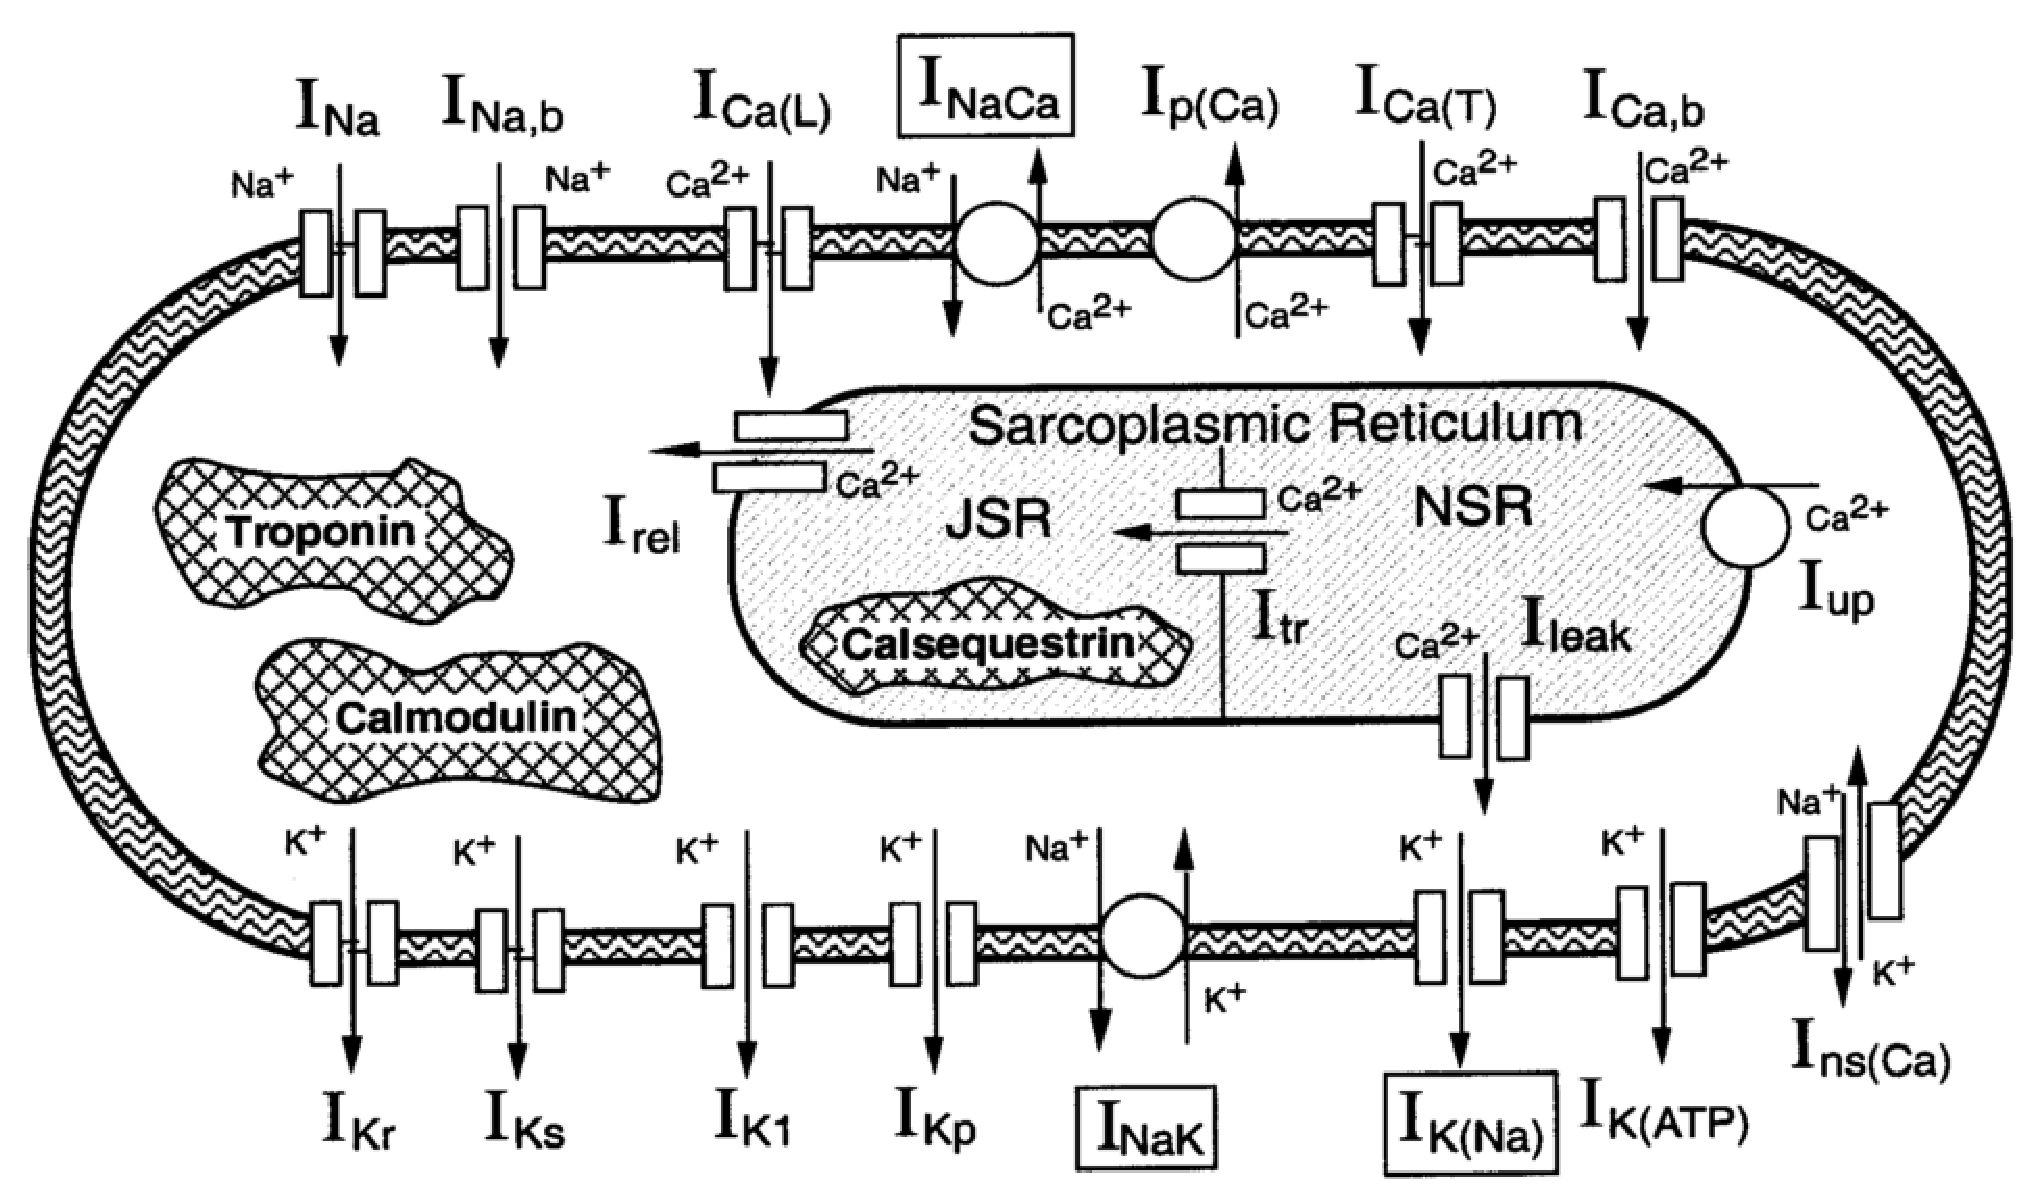
\includegraphics[height=5cm,
    angle=0]{./images/FaberRudy_cell.eps}}
\caption{RL2 model with some updates; $I_\ca$ becomes
  $I_{\ca(T)},I_{\ca(L)}$, $I_{\k}$ becomes $I_\Kr,I_\Ks$; and $I_{\k(\na)},I_{\k(ATP)}$}
\label{fig:FaberRudy_cell}
\end{figure}
Buffers: CaM and Troponin in myoplasm, and CSQN in SR. 

\section{Rudy (2000)}

\citep{rudy2000} used a Markovian model of the cardiac $\Na$ channel to
elucidate the mechanism of EAD through the inactivation and subsequent
re-activation of the L-type $\Ca$ channels. 

The effect of slow conduction was also examined by reducing the conductivity of
the gap junction, rather than through a loss of cellular excitability.

\section{Qu-\ldots-Weiss (2000) scroll wave}

\citep{qu2000}

\section{ten Tusscher-Noble-Noble-Panfilov (2004) (2D in human)}

Using the single-cell model described in Sect.\ref{sec:tenTusscher2004_human},
an important property of wave propagation in human ventricular tissue like
conduction velocity restitution (CVR) which is very important to occurence and
stability of reentrant arrhythmias \citep{qu1999} was studied.
Around that time, CVR data was only available from dog and guinea pig around
that time \citep{cao1999,girouard1996}.

\subsection{Hypothesis analysis}


\subsection{Mathematical model }

Spiral waves in 2D sheet of human ventricular tissue was done with membrane
potential recorded during spiral wave rotation. The 2D sheet of cardiac cells
was modelled as a continuous system with the PDE
\begin{equation}
C_m\frac{\partial V_m}{\partial t} = -I_\ion + I_\stim + \frac{1}{\rho_x S_x}
\frac{\partial^2 V_m}{\partial x^2} + \frac{1}{\rho_y S_y}
\frac{\partial^2 V_m}{\partial y^2} 
\end{equation}
with $\rho_x,\rho_y$ are cellular resistivity in x- and y-direction; $S_x,S_y$
are surface to volume ratio in the x- and y-direction. 
\begin{equation}
I_\ion = I_\na + I_{K1} + I_\to + I_\Kr + I_\Ks + I_\CaL + I_\NaCa + I_\NaK +
I_{pCa} + I_{pK} + I_\bCa + I_\bNa 
\end{equation}
with $I_{pCa},I_{pK}$ are plateau $\Ca$ and $\K$ currents.

In 1D simulation: Cell capacitance per unit area $C_m=2\muF/$cm$^2$,
surface-to-volume ratio $S=0.2$ per $\mum$ \citep{bernus2002}. 
To obtain a maximum planar conduction velocity (CV) of 70cm/s, the velocity
found for conductance along the fiber direction in human myocardium by
\citep{taggart2000}, they used a cellular resisistivity $\rho=162\Omega$cm,
which corresponds to the diffusion constant
$D=\frac{1}{\rho.S.C_m}=0.00154$cm$^2$/ms = 154$\mum^2/s$.

In 2D simulation: they assume isotropy diffusion, i.e. equal in all directions,
the same values were used for x- and y- direction as above. 


NOTE: The units being used are ms (time), mV (voltage), pA/pF (current density),
nS/pF (conductance $G_X$), mM (ion concentration). 

\subsection{Numerical method}

Forward Euler method was used with $\Delta x=0.1-0.2$ mm, and a time step of
$\Delta t = 0.01-0.02$ ms. However, this time step is too large to estimate the
Hodgkin-Huxley-type equations for the gating variables. For such values, they
used a different method: Rush-Larsen scheme \citep{rush1978pas}. In most
computational studies, they chose the smaller time step and smaller grid
size: $\Delta x=0.2$mm, $\Delta t=0.02$ms.


\subsection{Data analysis}

With $\Delta x=0.2mm$, decreasing $\Delta t=0.02$ms to 0.0025ms leads to an
increase of 3.7\% in CV. Similarly, using $\Delta t=0.02$ms, decreasing $\Delta
x=0.2$ to 0.1mm leads to an increase of 4.6\% in CV. The spatial and temporal
dependency of CV is similar to other models \citep{52}. However, it raised the
questions of computational stabilities, or whether equilibrium has reached. 


\section{Bondarenko-Rasmusson (2007)}

\citep{bondarenko2007}

\section{Bondarenko-Rasmusson (2009) - 2D tissue in mouse}

\citep{bondarenko2009}

\section{Xie-Sato-\ldots-Weiss (2010)}
\label{sec:xie-weiss2010}

When there is a big enough mismatch between the source/sink, the propagation
fails. \citep{xie2010sls} studied when early (EAD) and delayed (DAD) after
depolarization can overcome the source-sink mismatch. The mechanism to trigger
this premature ventricular complexes (PVC) in tissue is unclear.

%%% Local Variables: 
%%% mode: latex
%%% TeX-master: "mainfile"
%%% End: 
